\documentclass[french,12pt]{article}

%===============================================================================
% Packages
%===============================================================================
\usepackage[utf8]{inputenc}
\usepackage[T1]{fontenc}
\usepackage{lmodern}
\usepackage[margin=1.65cm]{geometry}
\usepackage{babel}
\usepackage{amsmath}
\usepackage{amssymb}
\usepackage{array}
\usepackage{graphicx}
\usepackage{xcolor}
\usepackage[most]{tcolorbox}
\usepackage{longtable}
\usepackage{hyperref}
\usepackage{caption}
\usepackage{transparent}
\usepackage{eso-pic}
\usepackage{listings}
\usepackage[section]{placeins}
\usepackage{subcaption}
\usepackage{float}
\usepackage{tikz}
\usetikzlibrary{shapes.geometric, arrows.meta, positioning}

%===============================================================================
% Configuration générale
%===============================================================================
\setlength{\parindent}{20pt}
\setlength{\parskip}{0.35em}
\renewcommand{\arraystretch}{1.18}
\sloppy

\hypersetup{
    colorlinks=true,
    linkcolor=blue!50!black,
    urlcolor=blue!50!black,
    citecolor=blue!50!black
}

\lstdefinestyle{codeStyle}{
    basicstyle=\ttfamily\small,
    breaklines=true,
    frame=single,
    backgroundcolor=\color{gray!8},
    keywordstyle=\color{blue!60!black},
    commentstyle=\color{green!40!black},
    stringstyle=\color{red!60!black},
    showstringspaces=false
}
\lstset{style=codeStyle}

%===============================================================================
% Fond de page compatible avec la structure fournie
%===============================================================================
\newcommand\BackgroundPic{%
\put(0,0){%
\parbox[b][\paperheight]{\paperwidth}{%
\vfill
\centering
\IfFileExists{images/background.png}{%
{\transparent{0.4}\includegraphics[width=\paperwidth,height=\paperheight]{images/background.png}}%
}{}%
\vfill
}}}

%===============================================================================
% Commande pour les figures optionnelles
%===============================================================================
\newcommand{\capture}[2]{%
\begin{figure}[htbp]
    \centering
    \IfFileExists{#1}{%
        \includegraphics[width=0.88\textwidth]{#1}%
    }{%
        \fbox{%
            \parbox[c][5.5cm][c]{0.85\textwidth}{%
                \centering \textbf{Figure optionnelle non trouvée}\\[0.3cm]
                #2\\[0.2cm]
                \texttt{#1}
            }%
        }%
    }
    \caption{#2}
\end{figure}
}

\begin{document}

\AddToShipoutPicture*{\BackgroundPic}

%%%%%%%%%%%%%%%%%%%%%%%%%%%%%%%%%%%%%%%%%%%%%%%%%%%%%%%%%%%%%%%%%%%%%%%%%%%%%%%%
% Page titre
%%%%%%%%%%%%%%%%%%%%%%%%%%%%%%%%%%%%%%%%%%%%%%%%%%%%%%%%%%%%%%%%%%%%%%%%%%%%%%%%
\begin{titlepage}
    \newcommand{\HRule}{\rule{\linewidth}{0.5mm}}
    \center

    \textsc{\LARGE Université du Québec à Chicoutimi}\\[1.5cm]
    \textsc{\Large Département d'informatique et de mathématique}\\[0.5cm]
    \textsc{\large 8INF934 -- Atelier pratique en intelligence artificielle I}\\[0.5cm]

    \HRule\\[0.5cm]
    {\huge\bfseries Aftermath : L'outil IA pour la détection et classification des bâtiments post-catastrophes}\\[0.2cm]
    {\large\itshape Voir les dégâts pour agir plus vite}\\[0.2cm]
    \HRule\\[0.5cm]

    \begin{center}
        \large
        \textit{Étudiants}\\
        Thomas GOURJAULT\\
        Grégory JOURDAIN\\
        Aurélien CASAGRANDI\\
        Matthis LAHARGOUE
    \end{center}

    \vspace{1cm}

    {\large\textit{Remis à}}\\
    Julien \textsc{MAITRE}

    \vfill\vfill\vfill
    {\large 16 juin 2026}

    \vfill\vfill
    \IfFileExists{images/logo_uqac.png}{%
        \includegraphics[width=0.2\textwidth]{images/logo_uqac.png}\\[1cm]
    }{%
        \vspace{1cm}
    }
    \vfill
\end{titlepage}

%%%%%%%%%%%%%%%%%%%%%%%%%%%%%%%%%%%%%%%%%%%%%%%%%%%%%%%%%%%%%%%%%%%%%%%%%%%%%%%%
% Table des matières
%%%%%%%%%%%%%%%%%%%%%%%%%%%%%%%%%%%%%%%%%%%%%%%%%%%%%%%%%%%%%%%%%%%%%%%%%%%%%%%%
\tableofcontents
\newpage

\section{Introduction}

\subsection{Problématique}

Lorsqu'une catastrophe naturelle majeure survient (séisme, ouragan, inondation, etc.), les premières heures sont cruciales pour organiser les secours et sauver des vies. Actuellement, l'évaluation des dégâts repose souvent sur des reconnaissances physiques au sol ou des analyses manuelles d'images satellites. Ces méthodes sont très lentes, ce qui retarde le déploiement de l'aide humanitaire là où elle est le plus nécessaire. Le dataset xBD a précisément été proposé pour répondre à ce type d'enjeu, en fournissant des images satellites avant et après catastrophe ainsi que des annotations de bâtiments et de niveaux de dommages \cite{xbd}.

La question à ce problème devient donc :
\begin{center}
\textit{Comment automatiser et accélérer l'évaluation spatiale des dommages structurels post-catastrophe à partir d'imagerie satellite ?}
\end{center}

Avec l'expansion de l'intelligence artificielle et des méthodes de vision par ordinateur, il devient possible d'automatiser une partie de cette analyse. C'est dans cette logique que nous avons conçu \textbf{Aftermath}, un outil simple d'utilisation permettant de transformer des images satellites en cartes de dégâts exploitables.

\begin{figure}[H]
    \centering
    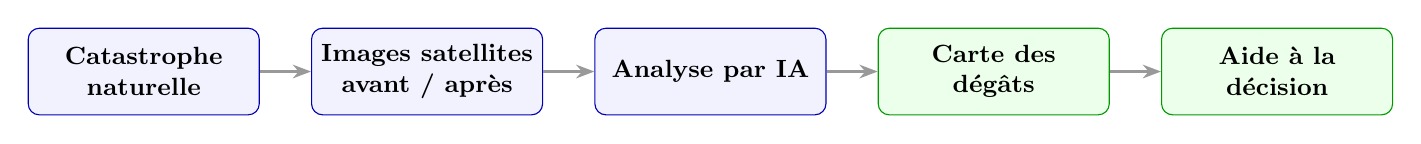
\begin{tikzpicture}[
        node distance=0.8cm and 0.65cm,
        box/.style={
            rectangle,
            draw=blue!70!black,
            fill=blue!5,
            rounded corners,
            minimum height=1.1cm,
            text width=2.7cm,
            align=center,
            font=\small\bfseries
        },
        output/.style={
            rectangle,
            draw=green!60!black,
            fill=green!8,
            rounded corners,
            minimum height=1.1cm,
            text width=2.7cm,
            align=center,
            font=\small\bfseries
        },
        arrow/.style={-Stealth, thick, draw=gray!80}
    ]

    \node (catastrophe) [box] {Catastrophe naturelle};
    \node (satellite) [box, right=of catastrophe] {Images satellites avant / après};
    \node (ia) [box, right=of satellite] {Analyse par IA};
    \node (carte) [output, right=of ia] {Carte des dégâts};
    \node (decision) [output, right=of carte] {Aide à la décision};

    \draw [arrow] (catastrophe) -- (satellite);
    \draw [arrow] (satellite) -- (ia);
    \draw [arrow] (ia) -- (carte);
    \draw [arrow] (carte) -- (decision);

    \end{tikzpicture}
    \caption{Principe général de la solution Aftermath : transformer des images satellites en information exploitable pour la gestion de crise.}
    \label{fig:principe_aftermath}
\end{figure}

\subsection{Objectifs}

Les objectifs de ce projet sont multiples :
\begin{enumerate}
    \item \textbf{Détection des bâtiments} : repérer les zones bâties afin de concentrer l'analyse sur les éléments réellement utiles pour les secours.
    \item \textbf{Classification des bâtiments} : déterminer le niveau d'endommagement afin d'aider à prioriser les zones d'intervention.
    \item \textbf{Création d'une interface simple} : proposer un support permettant à un utilisateur non expert en informatique d'utiliser facilement l'IA et d'interpréter simplement ses prédictions.
    \item \textbf{Comparaison des approches testées} : comparer une première approche \textit{baseline}, les différents modèles expérimentés et les approches existantes dans la littérature.
\end{enumerate}

\subsection{Bénéficiaires}

La solution développée dans ce projet s'adresse directement aux structures de gestion de crise et d'urgence humanitaire, telles que le \textbf{PAM}, l'\textbf{UNICEF}, les agences de l'\textbf{ONU}, la \textbf{Sécurité Civile}, les \textbf{assureurs} et les \textbf{collectivités locales}. L'outil vise à accélérer le déploiement des secours là où une analyse manuelle de la situation pouvait prendre plusieurs heures ou plusieurs jours. Les équipes terrain peuvent ainsi mieux orienter la logistique, tracer des itinéraires d'évacuation sécurisés et cibler en priorité les zones résidentielles les plus touchées.

Il est cependant important de préciser que les prédictions restent une sortie d'intelligence artificielle. Elles peuvent donc être fausses ou incomplètes. L'outil doit être considéré comme une aide à la décision, et non comme une vérité absolue.

\section{Données utilisées}

\subsection{Sources de données}

Pour mener à bien ce projet, nous exploitons le dataset de référence mondial xBD, issu du défi xView2. Ce jeu de données est spécifiquement conçu pour l'évaluation automatisée des dommages humanitaires par imagerie satellite haute résolution. Il fournit des images pré et post-catastrophe, des polygones de bâtiments et des labels ordinaux de niveaux de dégâts \cite{xbd}. Notre étude s'appuie plus précisément sur un volume de 2 799 paires d'images satellites brutes, capturées à la fois avant et après la catastrophe.

L'une des grandes richesses de ce dataset est sa diversité géographique et thématique. Il concerne plusieurs typologies de catastrophes naturelles réparties à travers le monde, incluant des phénomènes à déclenchement soudain comme des séismes au Mexique, des inondations dans le Midwest américain, des destructions par des ouragans et cyclones lors du passage de l'Ouragan Michael ou du Cyclone Idai, ainsi que des feux de forêt en Californie et des coulées de boue. Cette variété environnementale et architecturale permet d'exposer les modèles à des contextes visuels hétérogènes, ce qui renforce leur capacité de généralisation.

\begin{figure}[H]
    \centering
    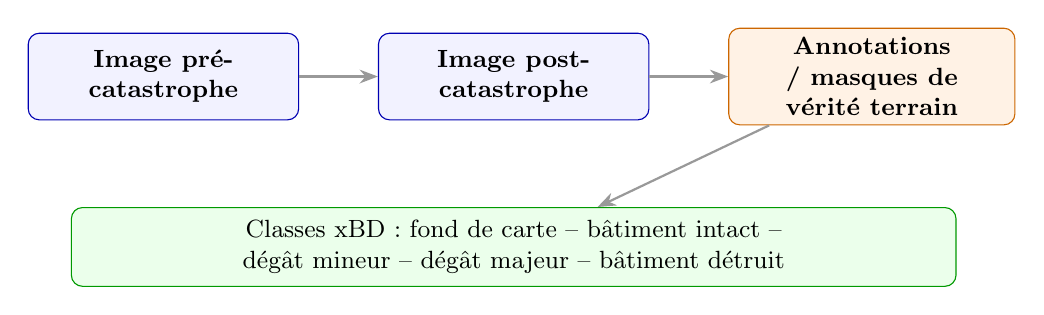
\begin{tikzpicture}[
        node distance=0.8cm and 1cm,
        data/.style={
            rectangle,
            draw=blue!70!black,
            fill=blue!5,
            rounded corners,
            minimum height=1.1cm,
            text width=3.2cm,
            align=center,
            font=\small\bfseries
        },
        label/.style={
            rectangle,
            draw=orange!80!black,
            fill=orange!10,
            rounded corners,
            minimum height=1.1cm,
            text width=3.4cm,
            align=center,
            font=\small\bfseries
        },
        class/.style={
            rectangle,
            draw=green!60!black,
            fill=green!8,
            rounded corners,
            minimum height=1cm,
            text width=11cm,
            align=center,
            font=\small
        },
        arrow/.style={-Stealth, thick, draw=gray!80}
    ]

    \node (pre) [data] {Image pré-catastrophe};
    \node (post) [data, right=of pre] {Image post-catastrophe};
    \node (mask) [label, right=of post] {Annotations / masques de vérité terrain};

    \node (classes) [class, below=of post, yshift=-0.3cm] {
        Classes xBD : fond de carte -- bâtiment intact -- dégât mineur -- dégât majeur -- bâtiment détruit
    };

    \draw [arrow] (pre) -- (post);
    \draw [arrow] (post) -- (mask);
    \draw [arrow] (mask) -- (classes);

    \end{tikzpicture}
    \caption{Structure d'une paire d'images du dataset xBD utilisée pour l'apprentissage supervisé.}
    \label{fig:structure_xbd}
\end{figure}

Voici un exemple de paire d'images brutes, concernant une éruption volcanique au Guatemala :
\begin{figure}[H]
  \centering
  \begin{subfigure}[b]{0.42\textwidth}
    \centering
    \IfFileExists{images/guatemala-volcano_00000000_pre_disaster.png}{%
        \includegraphics[width=\textwidth]{images/guatemala-volcano_00000000_pre_disaster.png}%
    }{%
        \fbox{\parbox[c][4.5cm][c]{0.95\textwidth}{\centering Image pré-catastrophe à insérer}}
    }
    \caption{Image satellite pré-catastrophe}
  \end{subfigure}
  \hfill
  \begin{subfigure}[b]{0.42\textwidth}
    \centering
    \IfFileExists{images/guatemala-volcano_00000000_post_disaster.png}{%
        \includegraphics[width=\textwidth]{images/guatemala-volcano_00000000_post_disaster.png}%
    }{%
        \fbox{\parbox[c][4.5cm][c]{0.95\textwidth}{\centering Image post-catastrophe à insérer}}
    }
    \caption{Image satellite post-catastrophe}
  \end{subfigure}
  \caption{Exemple d'une paire d'images satellites pré et post-catastrophe issue du dataset xBD.}
  \label{fig:exemple_guatemala}
\end{figure}

\subsection{Analyse exploratoire}

L'analyse exploratoire des données met en lumière deux défis majeurs liés à la structure intrinsèque de l'imagerie satellite de crise : la répartition de la sévérité des dégâts et la distribution spatiale des pixels.

Tout d'abord, l'étude du dataset xBD montre que les bâtiments post-catastrophe peuvent être associés à plusieurs classes : bâtiment intact, dégât mineur, dégât majeur, bâtiment détruit et cas non classifié. Pour l'apprentissage par masque, une classe de fond est également nécessaire afin de distinguer les zones non bâties des zones utiles à l'analyse.

L'examen des données révèle ensuite un déséquilibre de classes particulièrement marqué. Sur l'ensemble des images, une grande majorité de la surface est occupée par la classe de fond : forêts, routes, champs, océans ou zones non bâties. Les bâtiments ne représentent qu'une faible partie des pixels totaux et, au sein même de cette catégorie, les bâtiments associés à des dégâts majeurs ou à une destruction complète constituent un signal encore plus rare et localisé. Ce déséquilibre pose un risque direct : un modèle naïf pourrait maximiser son exactitude globale en prédisant majoritairement le fond, tout en échouant sur les classes de dommages qui sont pourtant les plus importantes opérationnellement. Ce constat est cohérent avec les difficultés décrites dans les travaux sur xBD et xView2, où l'évaluation automatique des dégâts repose sur un signal spatial rare, localisé et fortement déséquilibré \cite{xbd,xview2_multitemporal}.

\begin{figure}[H]
    \centering
    \IfFileExists{images/eda_disaster_distribution.png}{%
        \includegraphics[width=0.9\textwidth]{images/eda_disaster_distribution.png}
    }{%
        \fbox{\parbox[c][5cm][c]{0.9\textwidth}{\centering Distribution des catastrophes à insérer}}
    }
    \caption{Distribution des paires d'images selon les catastrophes présentes dans le dataset xBD.}
    \label{fig:eda_disaster_distribution}
\end{figure}

\begin{figure}[H]
    \centering
    \IfFileExists{images/eda_damage_distribution.png}{%
        \includegraphics[width=0.85\textwidth]{images/eda_damage_distribution.png}
    }{%
        \fbox{\parbox[c][5cm][c]{0.85\textwidth}{\centering Distribution des classes de dommages à insérer}}
    }
    \caption{Répartition des classes de dommages dans les annotations post-catastrophe.}
    \label{fig:eda_damage_distribution}
\end{figure}

\begin{figure}[H]
    \centering
    \IfFileExists{images/eda_target_pixel_distribution.png}{%
        \includegraphics[width=0.85\textwidth]{images/eda_target_pixel_distribution.png}
    }{%
        \fbox{\parbox[c][5cm][c]{0.85\textwidth}{\centering Distribution des pixels des masques à insérer}}
    }
    \caption{Distribution des valeurs de pixels dans les masques cibles.}
    \label{fig:eda_target_pixel_distribution}
\end{figure}

Ainsi, pour compenser ce déséquilibre, nous avons eu recours à plusieurs techniques : augmentation de données, filtrage qualitatif des images d'entraînement et choix de fonctions de perte adaptées aux classes rares. Ces choix sont détaillés dans la suite du rapport.

\section{Méthodes d'intelligence artificielle}

\subsection{Choix méthodologiques}

Le problème étudié relève de la segmentation sémantique : l'objectif n'est pas seulement de classer une image entière, mais d'attribuer une classe à chaque pixel. Dans notre cas, le modèle doit localiser les bâtiments et déterminer leur état après une catastrophe. Les architectures de type U-Net sont adaptées à ce type de tâche, car elles combinent une phase d'encodage pour extraire le contexte visuel et une phase de décodage pour reconstruire une carte de prédiction localisée \cite{unet}.

Le projet repose également sur une contrainte spécifique : les informations importantes ne se trouvent pas seulement dans l'image post-catastrophe, mais dans la comparaison entre l'état avant et l'état après. Une image post-catastrophe seule peut être ambiguë : un terrain vide peut être une zone naturellement non bâtie ou l'emplacement d'un bâtiment détruit. L'utilisation d'une paire d'images permet donc de raisonner en termes de changement temporel, ce qui est central pour l'évaluation automatique des dommages \cite{xview2_multitemporal}.

\subsection{Algorithmes étudiés}

Plusieurs familles d'approches ont été considérées. Une première approche de type \textit{baseline} consiste à utiliser un modèle U-Net classique pour produire une segmentation dense. Cette approche est simple, robuste et constitue un point de comparaison utile, mais elle ne tire pas toujours pleinement parti de la relation temporelle entre l'image avant et l'image après.

Nous avons ensuite étudié des architectures inspirées de U-Net++ et des modèles siamois. U-Net++ améliore l'architecture U-Net classique grâce à des connexions de saut imbriquées, conçues pour réduire l'écart sémantique entre les caractéristiques de l'encodeur et celles du décodeur \cite{unetplusplus}. Les approches siamoises, quant à elles, utilisent deux branches pour traiter conjointement les images pré et post-catastrophe. Des travaux réalisés sur xView2 ont montré l'intérêt de la fusion multi-temporelle et de modèles de type Siam-U-Net-Attn pour l'évaluation des dégâts à partir de paires d'images satellites \cite{xview2_multitemporal,siamunet_attn}.

\subsection{Méthode retenue}

La méthode retenue repose sur une logique siamoise : les images avant et après catastrophe sont traitées conjointement afin d'apprendre directement les changements temporels. Le modèle cherche donc à isoler les différences pertinentes entre les deux images plutôt qu'à analyser uniquement la scène finale. Cette stratégie est adaptée au contexte de xBD, où les labels de dommages sont liés à l'évolution des bâtiments entre deux dates \cite{xbd,xview2_multitemporal}.

\begin{figure}[H]
    \centering
    \resizebox{0.86\textwidth}{!}{%
    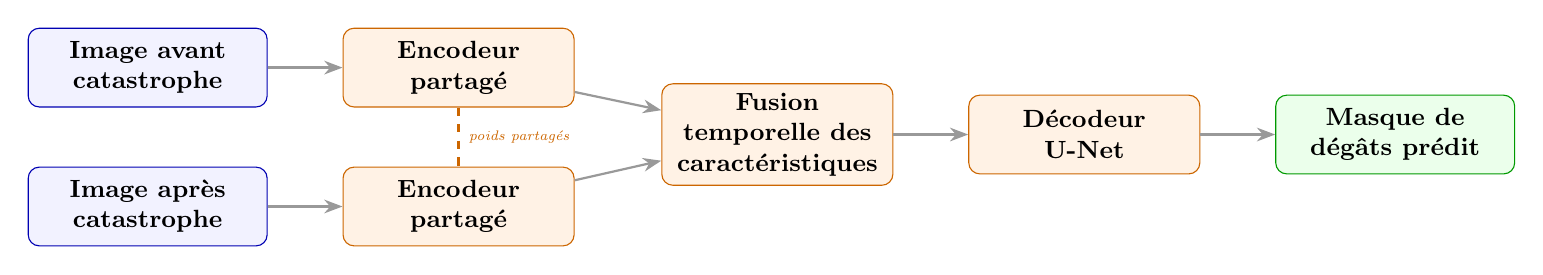
\begin{tikzpicture}[
        node distance=0.75cm and 0.95cm,
        input/.style={
            rectangle,
            draw=blue!70!black,
            fill=blue!5,
            rounded corners,
            minimum height=1cm,
            text width=2.8cm,
            align=center,
            font=\small\bfseries
        },
        model/.style={
            rectangle,
            draw=orange!80!black,
            fill=orange!10,
            rounded corners,
            minimum height=1cm,
            text width=2.7cm,
            align=center,
            font=\small\bfseries
        },
        output/.style={
            rectangle,
            draw=green!60!black,
            fill=green!8,
            rounded corners,
            minimum height=1cm,
            text width=2.8cm,
            align=center,
            font=\small\bfseries
        },
        arrow/.style={-Stealth, thick, draw=gray!80}
    ]

    \node (pre) [input] {Image avant catastrophe};
    \node (post) [input, below=of pre] {Image après catastrophe};

    \node (encpre) [model, right=of pre] {Encodeur partagé};
    \node (encpost) [model, right=of post] {Encodeur partagé};

    \node (fusion) [model, right=1.1cm of encpre, yshift=-0.85cm] {Fusion temporelle des caractéristiques};
    \node (decoder) [model, right=of fusion] {Décodeur U-Net};
    \node (mask) [output, right=of decoder] {Masque de dégâts prédit};

    \draw [arrow] (pre) -- (encpre);
    \draw [arrow] (post) -- (encpost);
    \draw [arrow] (encpre) -- (fusion);
    \draw [arrow] (encpost) -- (fusion);
    \draw [arrow] (fusion) -- (decoder);
    \draw [arrow] (decoder) -- (mask);

    \draw [dashed, thick, draw=orange!80!black] (encpre) -- (encpost)
        node[midway, right, font=\tiny\itshape, text=orange!80!black] {poids partagés};

    \end{tikzpicture}
    }
    \caption{Principe de l'architecture Siamese U-Net utilisée pour comparer les images avant et après catastrophe.}
    \label{fig:siamese_unet}
\end{figure}


Pour la gestion du déséquilibre de classes, les fonctions de perte de type Dice ou Tversky sont particulièrement pertinentes, car elles permettent de mieux prendre en compte les petites régions segmentées lorsque les pixels utiles sont rares par rapport au fond \cite{dice_loss,tversky_loss,focal_tversky}.

\section{Architecture de la solution}

\subsection{Pipeline de traitement}

\begin{figure}[H]
    \centering
    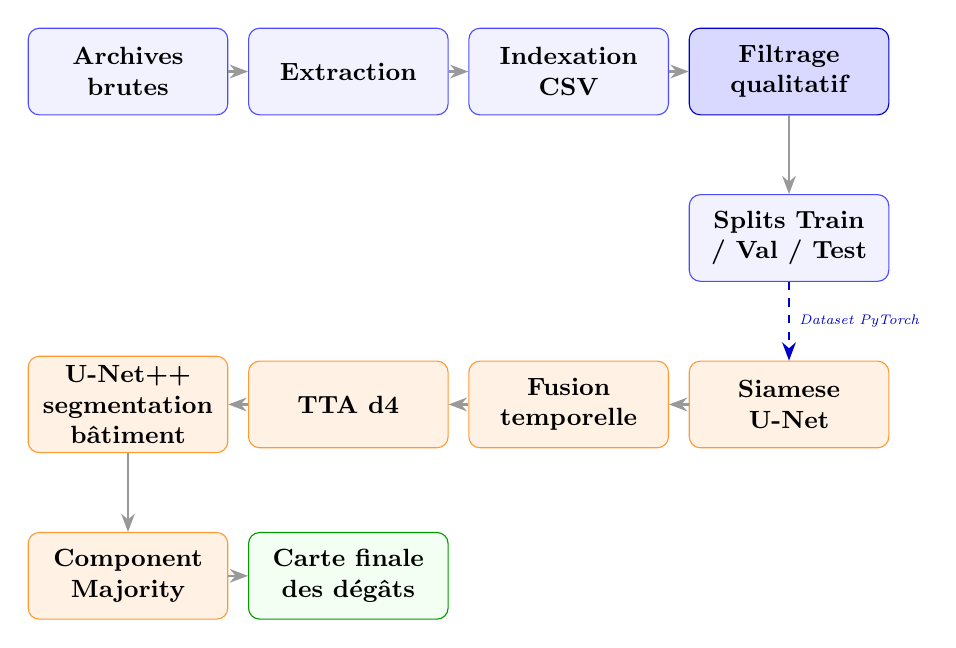
\begin{tikzpicture}[
        node distance=0.6cm and 0.25cm,
        process/.style={
            rectangle,
            draw=blue!70,
            fill=blue!5,
            text width=2.3cm,
            minimum height=1.1cm,
            align=center,
            rounded corners,
            font=\small\bfseries
        },
        model/.style={
            rectangle,
            draw=orange!80,
            fill=orange!10,
            text width=2.3cm,
            minimum height=1.1cm,
            align=center,
            rounded corners,
            font=\small\bfseries
        },
        output/.style={
            rectangle,
            draw=green!60!black,
            fill=green!5,
            text width=2.3cm,
            minimum height=1.1cm,
            align=center,
            rounded corners,
            font=\small\bfseries
        },
        arrow/.style={-Stealth, thick, draw=gray!80}
    ]

    \node (extract)  [process] at (0,0) {Extraction};
    \node (brutes)   [process, left=of extract] {Archives brutes};
    \node (csv)      [process, right=of extract] {Indexation CSV};
    \node (filtrage) [process, right=of csv, draw=blue!80!black, fill=blue!15] {Filtrage qualitatif};

    \node (splits)   [process, below=of filtrage, yshift=-0.4cm] {Splits Train / Val / Test};

    \node (siamese)  [model, below=of splits, yshift=-0.4cm] {Siamese U-Net};
    \node (fusion)   [model, left=of siamese] {Fusion temporelle};
    \node (tta)      [model, left=of fusion] {TTA d4};
    \node (building) [model, left=of tta] {U-Net++ segmentation bâtiment};

    \node (majority) [model, below=of building, yshift=-0.4cm] {Component Majority};
    \node (carte)    [output, right=of majority] {Carte finale des dégâts};

    \draw [arrow] (brutes) -- (extract);
    \draw [arrow] (extract) -- (csv);
    \draw [arrow] (csv) -- (filtrage);
    \draw [arrow] (filtrage) -- (splits);
    \draw [arrow, dashed, draw=blue!80!black] (splits) -- (siamese)
        node[pos=0.5, right, font=\tiny\itshape, text=blue!80!black] {Dataset PyTorch};
    \draw [arrow] (siamese) -- (fusion);
    \draw [arrow] (fusion) -- (tta);
    \draw [arrow] (tta) -- (building);
    \draw [arrow] (building) -- (majority);
    \draw [arrow] (majority) -- (carte);

    \end{tikzpicture}
    \caption{Pipeline global unifié : de la préparation des archives brutes à la génération de la carte finale des dégâts.}
    \label{fig:pipeline_global}
\end{figure}

Comme l'illustre la figure~\ref{fig:pipeline_global}, l'ensemble du projet est structuré autour d'un flux de traitement unifié qui relie la préparation des données à l'analyse par l'intelligence artificielle.

La première phase prend en charge le traitement des données brutes du dataset xBD. Après l'extraction et l'indexation dans un CSV, les images subissent un filtrage qualitatif afin de privilégier les images utiles pour l'entraînement, avant d'être découpées en sous-ensembles d'entraînement, de validation et de test. Ce processus génère le dataset PyTorch final.

La seconde phase concerne la chaîne de prédiction. Les paires d'images entrent dans le modèle Siamese U-Net pour isoler les changements temporels. Les prédictions obtenues sont ensuite stabilisées par l'algorithme TTA d4, puis croisées avec les masques du modèle U-Net++ afin de cibler uniquement les bâtiments et d'éviter les fausses détections sur le décor. Enfin, après un lissage par décision majoritaire de la classe par bâtiment, le système génère la carte finale des dégâts.

\subsection{Post-traitement par décision majoritaire}

Après la prédiction pixel par pixel, certaines zones peuvent contenir du bruit : un même bâtiment peut être partiellement classé comme intact et partiellement comme endommagé. Pour obtenir une sortie plus cohérente, nous appliquons un post-traitement par \textit{component majority}. Le principe consiste à identifier chaque bâtiment comme une composante connectée, puis à lui attribuer la classe majoritaire prédite parmi ses pixels.

\begin{figure}[H]
    \centering
    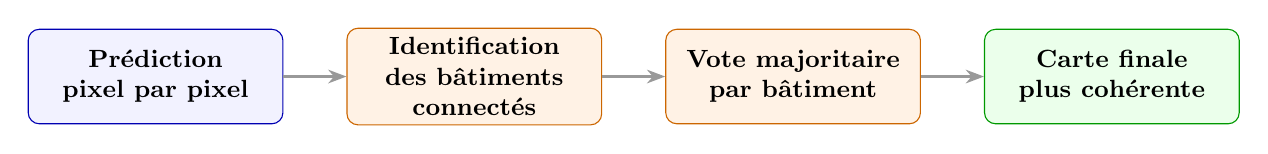
\begin{tikzpicture}[
        node distance=0.8cm and 0.8cm,
        stepbox/.style={
            rectangle,
            draw=blue!70!black,
            fill=blue!5,
            rounded corners,
            minimum height=1.2cm,
            text width=3cm,
            align=center,
            font=\small\bfseries
        },
        process/.style={
            rectangle,
            draw=orange!80!black,
            fill=orange!10,
            rounded corners,
            minimum height=1.2cm,
            text width=3cm,
            align=center,
            font=\small\bfseries
        },
        output/.style={
            rectangle,
            draw=green!60!black,
            fill=green!8,
            rounded corners,
            minimum height=1.2cm,
            text width=3cm,
            align=center,
            font=\small\bfseries
        },
        arrow/.style={-Stealth, thick, draw=gray!80}
    ]

    \node (pred) [stepbox] {Prédiction pixel par pixel};
    \node (components) [process, right=of pred] {Identification des bâtiments connectés};
    \node (vote) [process, right=of components] {Vote majoritaire par bâtiment};
    \node (final) [output, right=of vote] {Carte finale plus cohérente};

    \draw [arrow] (pred) -- (components);
    \draw [arrow] (components) -- (vote);
    \draw [arrow] (vote) -- (final);

    \end{tikzpicture}
    \caption{Principe du post-traitement par \textit{component majority} pour lisser les prédictions bâtiment par bâtiment.}
    \label{fig:component_majority}
\end{figure}

\subsection{Technologies utilisées}

\begin{table}[H]
    \centering
    \begin{tabular}{|>{\centering\arraybackslash}m{3.2cm}|>{\centering\arraybackslash}m{3.8cm}|>{\centering\arraybackslash}m{6.5cm}|}
        \hline
        \textbf{Module} & \textbf{Technologie / Outil} & \textbf{Justification} \\
        \hline
        Langage principal & Python & Standard en IA et compatible avec les bibliothèques du projet. \\ \hline
        Framework d'IA & PyTorch \cite{pytorch} & Flexibilité pour coder le modèle siamois et gestion native du calcul GPU. \\ \hline
        Déséquilibre des classes & Data augmentation / \hyperref[subsec:tta]{TTA} & Enrichit le jeu de données et stabilise les prédictions sur les bâtiments endommagés. \\ \hline
        Modélisation \& Architecture & U-Net siamois / U-Net++ EfficientNet-B4 \cite{unet,unetplusplus} & Capture les changements avant/après et isole précisément le contour des bâtiments. \\ \hline
        Gestion des données & Pandas, NumPy & Manipulation rapide des fichiers d'indexation CSV et calculs sur les matrices d'images. \\ \hline
        Calcul intensif & Cluster Rorqual (Alliance) & Puissance GPU indispensable pour l'entraînement à grande échelle. \\ \hline
        Orchestration GPU & SLURM \cite{slurm} & Planification et réservation des ressources de calcul sur le cluster. \\ \hline
        Interface utilisateur & Streamlit \cite{streamlit} & Création rapide d'une application web interactive. \\ \hline
    \end{tabular}
    \caption{Synthèse et justification des choix technologiques du projet.}
    \label{tab:technos}
\end{table}

\subsection{Paramètres}

Afin d'assurer la reproductibilité de nos expériences, les différents choix de configuration, les hyperparamètres ainsi que les ressources matérielles mobilisées pour l'entraînement du modèle sont synthétisés dans le tableau~\ref{tab:parametres_entrainement}.

\begin{table}[H]
    \centering
    \begin{tabular}{|c|>{\centering\arraybackslash}m{9.5cm}|}
        \hline
        \textbf{Configuration} & \textbf{Valeurs et caractéristiques} \\
        \hline
        Taille du jeu de données & 2 799 paires d'images satellites, découpées en tuiles utiles \\ \hline
        Répartition du split & Train / validation / test selon le protocole expérimental retenu \\ \hline
        Taille des images & $512 \times 512$ pixels (baseline) / $1024 \times 1024$ pixels (modèle long) \\ \hline
        Optimiseur et learning rate & AdamW et apprentissage de l'ordre de $10^{-4}$ à $2 \times 10^{-4}$ selon les campagnes retenues \\ \hline
        Taille de batch & Batch size 2 pour les images $1024 \times 1024$, afin de rester compatible avec les contraintes mémoire GPU \\ \hline
        Fonctions de perte (\textit{Loss}) & Focal-Tversky pour le champion damage, focal-Tversky pour le modèle bâtiment, et CE-Dice pour les baselines \cite{dice_loss,tversky_loss,focal_tversky} \\ \hline
        Métrique de validation clé & Mean IoU et IoU spécifique aux bâtiments endommagés \\ \hline
        Critères d'arrêt & Comparaison sur validation puis évaluation finale sur test; le modèle intégré est retenu pour sa stabilité, sa portabilité et ses métriques finales \\ \hline
        Ressources matérielles & GPU Nvidia H100 sur le cluster Rorqual d'Alliance pour les campagnes lourdes \\ \hline
    \end{tabular}
    \caption{Synthèse des paramètres et de l'environnement d'entraînement.}
    \label{tab:parametres_entrainement}
\end{table}

\subsection{Interface}

Le prototype final est une application Streamlit unique située dans \texttt{app/streamlit\_app.py}. Le rendu final conserve cette application stable, facile à installer et cohérente avec le dépôt GitHub. L'objectif de l'interface n'est pas de remplacer un système SIG complet, mais de démontrer une chaîne IA bout-en-bout : charger deux images satellites, exécuter le modèle, visualiser les masques intermédiaires, interpréter le résultat et exporter les éléments utiles à une analyse humaine.

L'application finale repose sur les checkpoints portables inclus dans le dépôt :
\begin{itemize}
    \item \texttt{outputs/checkpoints/dftv2\_hist1000\_attention\_sqrt2\_ft\_250\_seed0/best\_damage\_arch\_portable.pt} pour le modèle damage;
    \item \texttt{outputs/checkpoints/b400\_effb4\_sampler8\_ft/best\_building\_portable.pt} pour le modèle building.
\end{itemize}

\subsubsection{Sources d'images disponibles}

Trois modes de chargement sont disponibles. Le premier, \textbf{Exemples inclus}, utilise des paires pré/post-catastrophe embarquées dans \texttt{sample\_data/demo\_pairs/}; il permet à un évaluateur de lancer la démonstration sans télécharger le dataset complet xBD. Le second, \textbf{Upload manuel}, permet de téléverser une image avant catastrophe et une image après catastrophe au format PNG ou JPEG. Le troisième, \textbf{Dataset xBD optionnel}, reste disponible lorsque le dataset complet est présent localement; il sert surtout aux tests de recherche et à la comparaison avec la vérité terrain.

\subsubsection{Pipeline d'inférence}
\label{subsec:tta}

Le pipeline recommandé pour la démonstration combine plusieurs briques. Le modèle principal de damage est un \textbf{Siamese Attention} entraîné en 3 classes : fond, bâtiment intact et bâtiment endommagé. L'inférence peut être stabilisée par \textbf{TTA d4}, c'est-à-dire les huit transformations du groupe diédral : rotations et retournements appliqués au tenseur d'entrée, puis inversion et moyenne des logits avant l'argmax final. Ensuite, un modèle de segmentation bâtiment \textbf{U-Net++ EfficientNet-B4} prédit un masque binaire de bâtiments à partir de l'image pré-catastrophe. Le post-traitement \textit{component majority} applique enfin une décision majoritaire par composante bâtiment afin de rendre la carte plus cohérente spatialement.

L'utilisateur peut choisir entre un mode plus rapide et un mode de qualité maximale. Le mode recommandé pour la présentation est \textbf{damage + TTA d4 + segmentation bâtiment + component majority}, car il exploite les deux meilleurs modèles stabilisés dans le dépôt final.

\subsubsection{Visualisation et explicabilité}

L'onglet de visualisation affiche explicitement les éléments nécessaires à l'interprétation :
\begin{itemize}
    \item l'image avant catastrophe;
    \item l'image après catastrophe;
    \item le masque damage brut produit par le modèle;
    \item le masque bâtiment prédit;
    \item le masque damage final après post-traitement;
    \item l'overlay final superposé à l'image post-catastrophe;
    \item la vérité terrain lorsque l'exemple xBD la fournit.
\end{itemize}

Cette visualisation donne une forme d'explicabilité visuelle. Elle ne prétend pas expliquer tous les mécanismes internes du réseau de neurones, mais elle montre comment la prédiction finale est construite : prédiction damage, localisation bâtiment, correction par composantes et superposition finale.

\subsubsection{Métriques, incertitude et export}

Lorsque la vérité terrain est disponible, l'application calcule les métriques de segmentation sur la prédiction finale. En mode upload, où aucune vérité terrain n'est fournie, elle affiche plutôt des statistiques descriptives : surface prédite comme bâtiment, part endommagée et distribution des classes. L'onglet incertitude affiche une carte d'entropie basée sur les probabilités du modèle damage.

Les exports actuels du prototype sont volontairement simples : \textbf{PNG} pour les masques et overlays, et \textbf{JSON} pour les statistiques et métadonnées de l'analyse. Le prototype ne génère pas encore de GeoJSON, GeoTIFF, Shapefile, projet QGIS/ArcGIS, API publique ou géoréférencement opérationnel. Ces éléments sont documentés comme perspectives futures.

\begin{figure}[H]
    \centering
    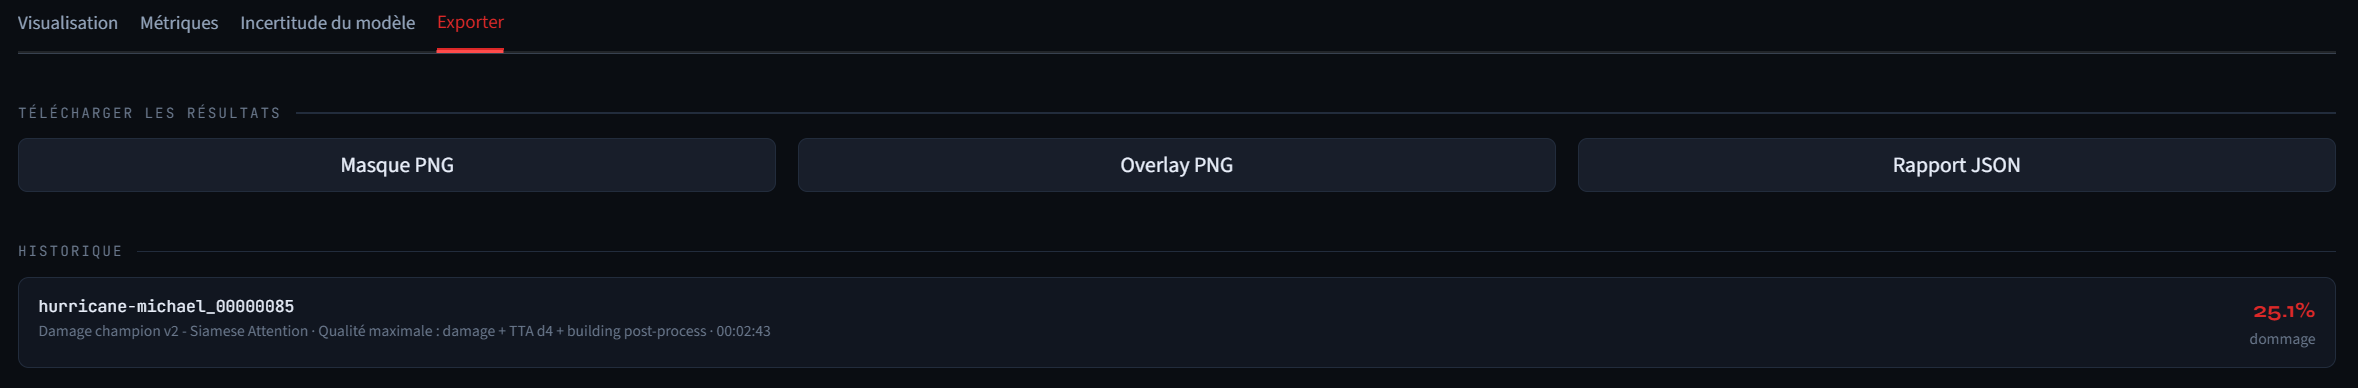
\includegraphics[width=0.9\textwidth]{docs/final_delivery/report_figures/app_exports.png}
    \caption{Onglet d'export de l'application finale. Les exports disponibles dans le prototype sont les masques et overlays en PNG, ainsi qu'un rapport JSON descriptif.}
    \label{fig:app_exports}
\end{figure}

\begin{figure}[H]
    \centering
    \begin{subfigure}[b]{0.48\textwidth}
        \centering
        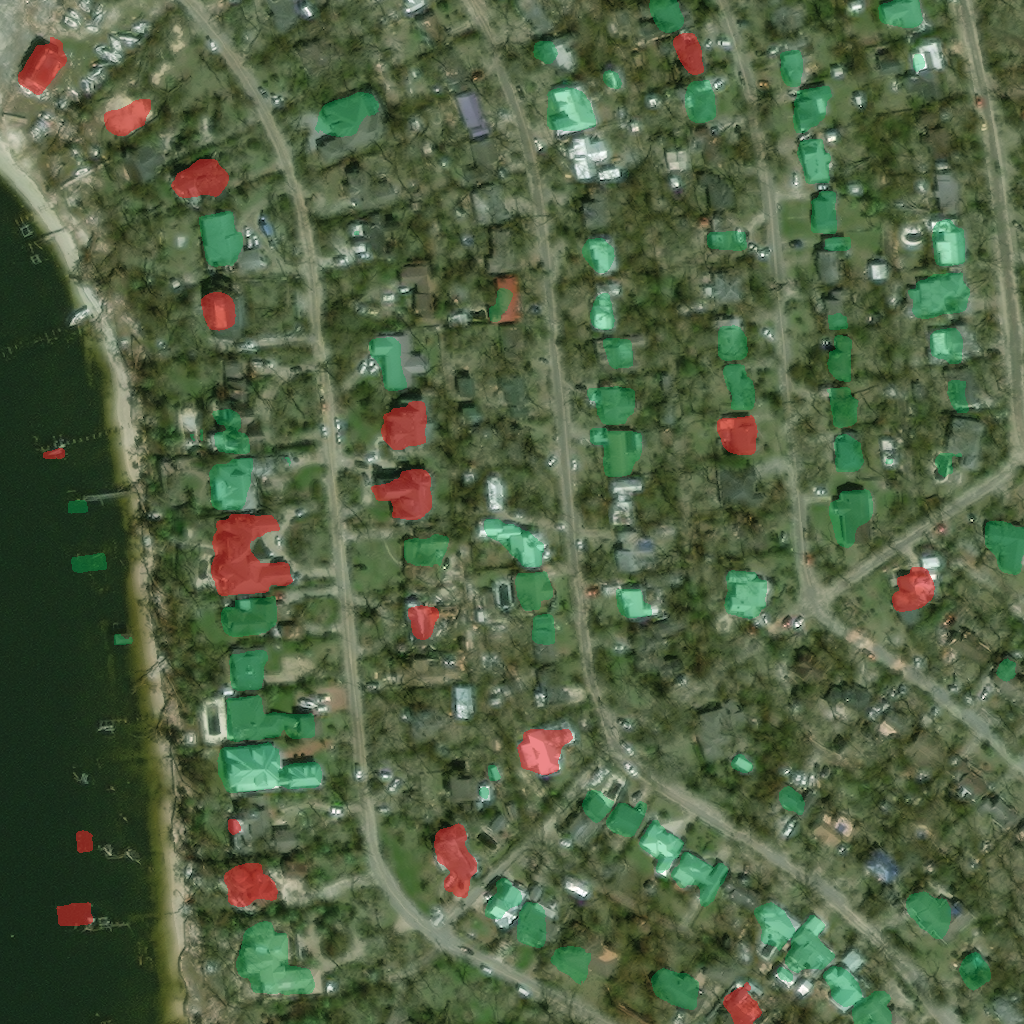
\includegraphics[width=\textwidth]{docs/final_delivery/report_figures/overlay_hurricane_michael_00000085.png}
        \caption{Overlay final exporté}
    \end{subfigure}
    \hfill
    \begin{subfigure}[b]{0.48\textwidth}
        \centering
        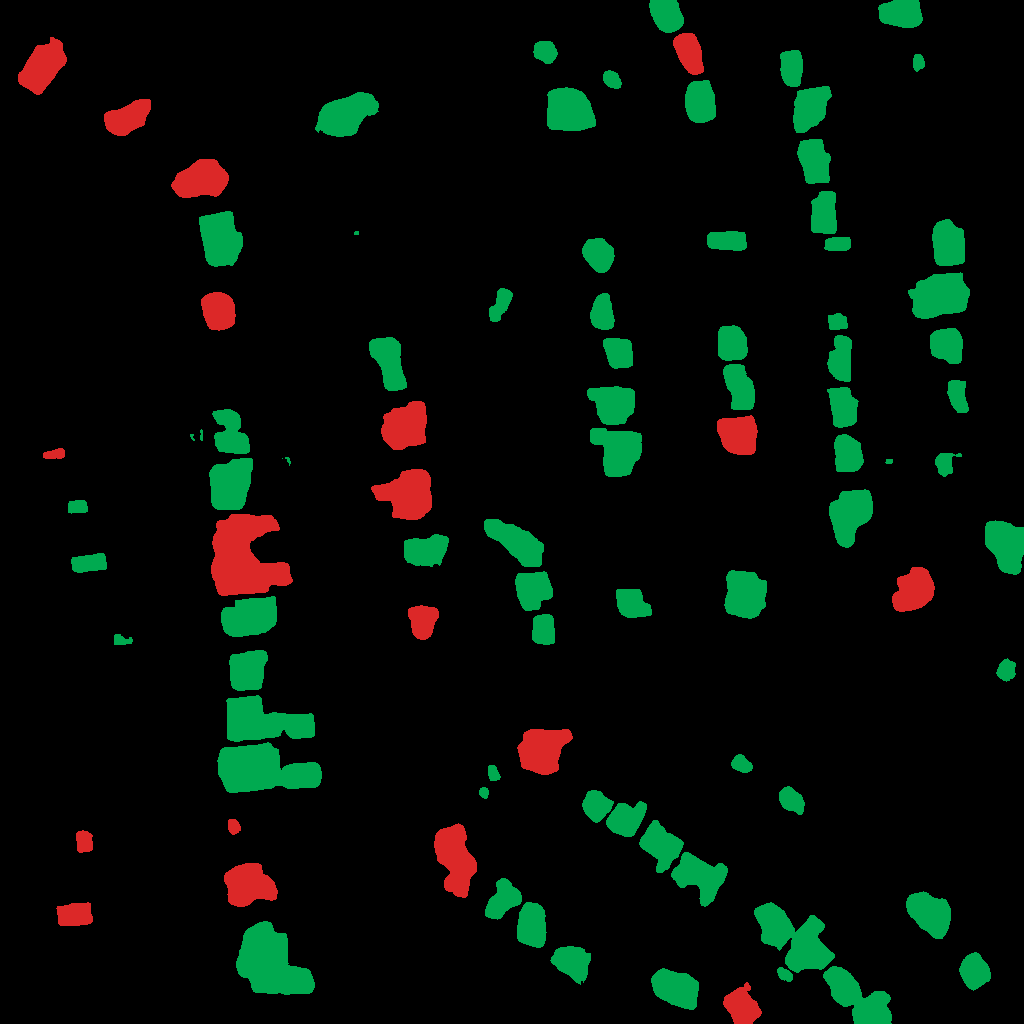
\includegraphics[width=\textwidth]{docs/final_delivery/report_figures/mask_hurricane_michael_00000085.png}
        \caption{Masque final exporté}
    \end{subfigure}
    \caption{Exemples d'exports PNG produits par l'application pour la paire \texttt{hurricane-michael\_00000085}.}
    \label{fig:exports_png_hurricane_michael}
\end{figure}

\begin{figure}[H]
    \centering
    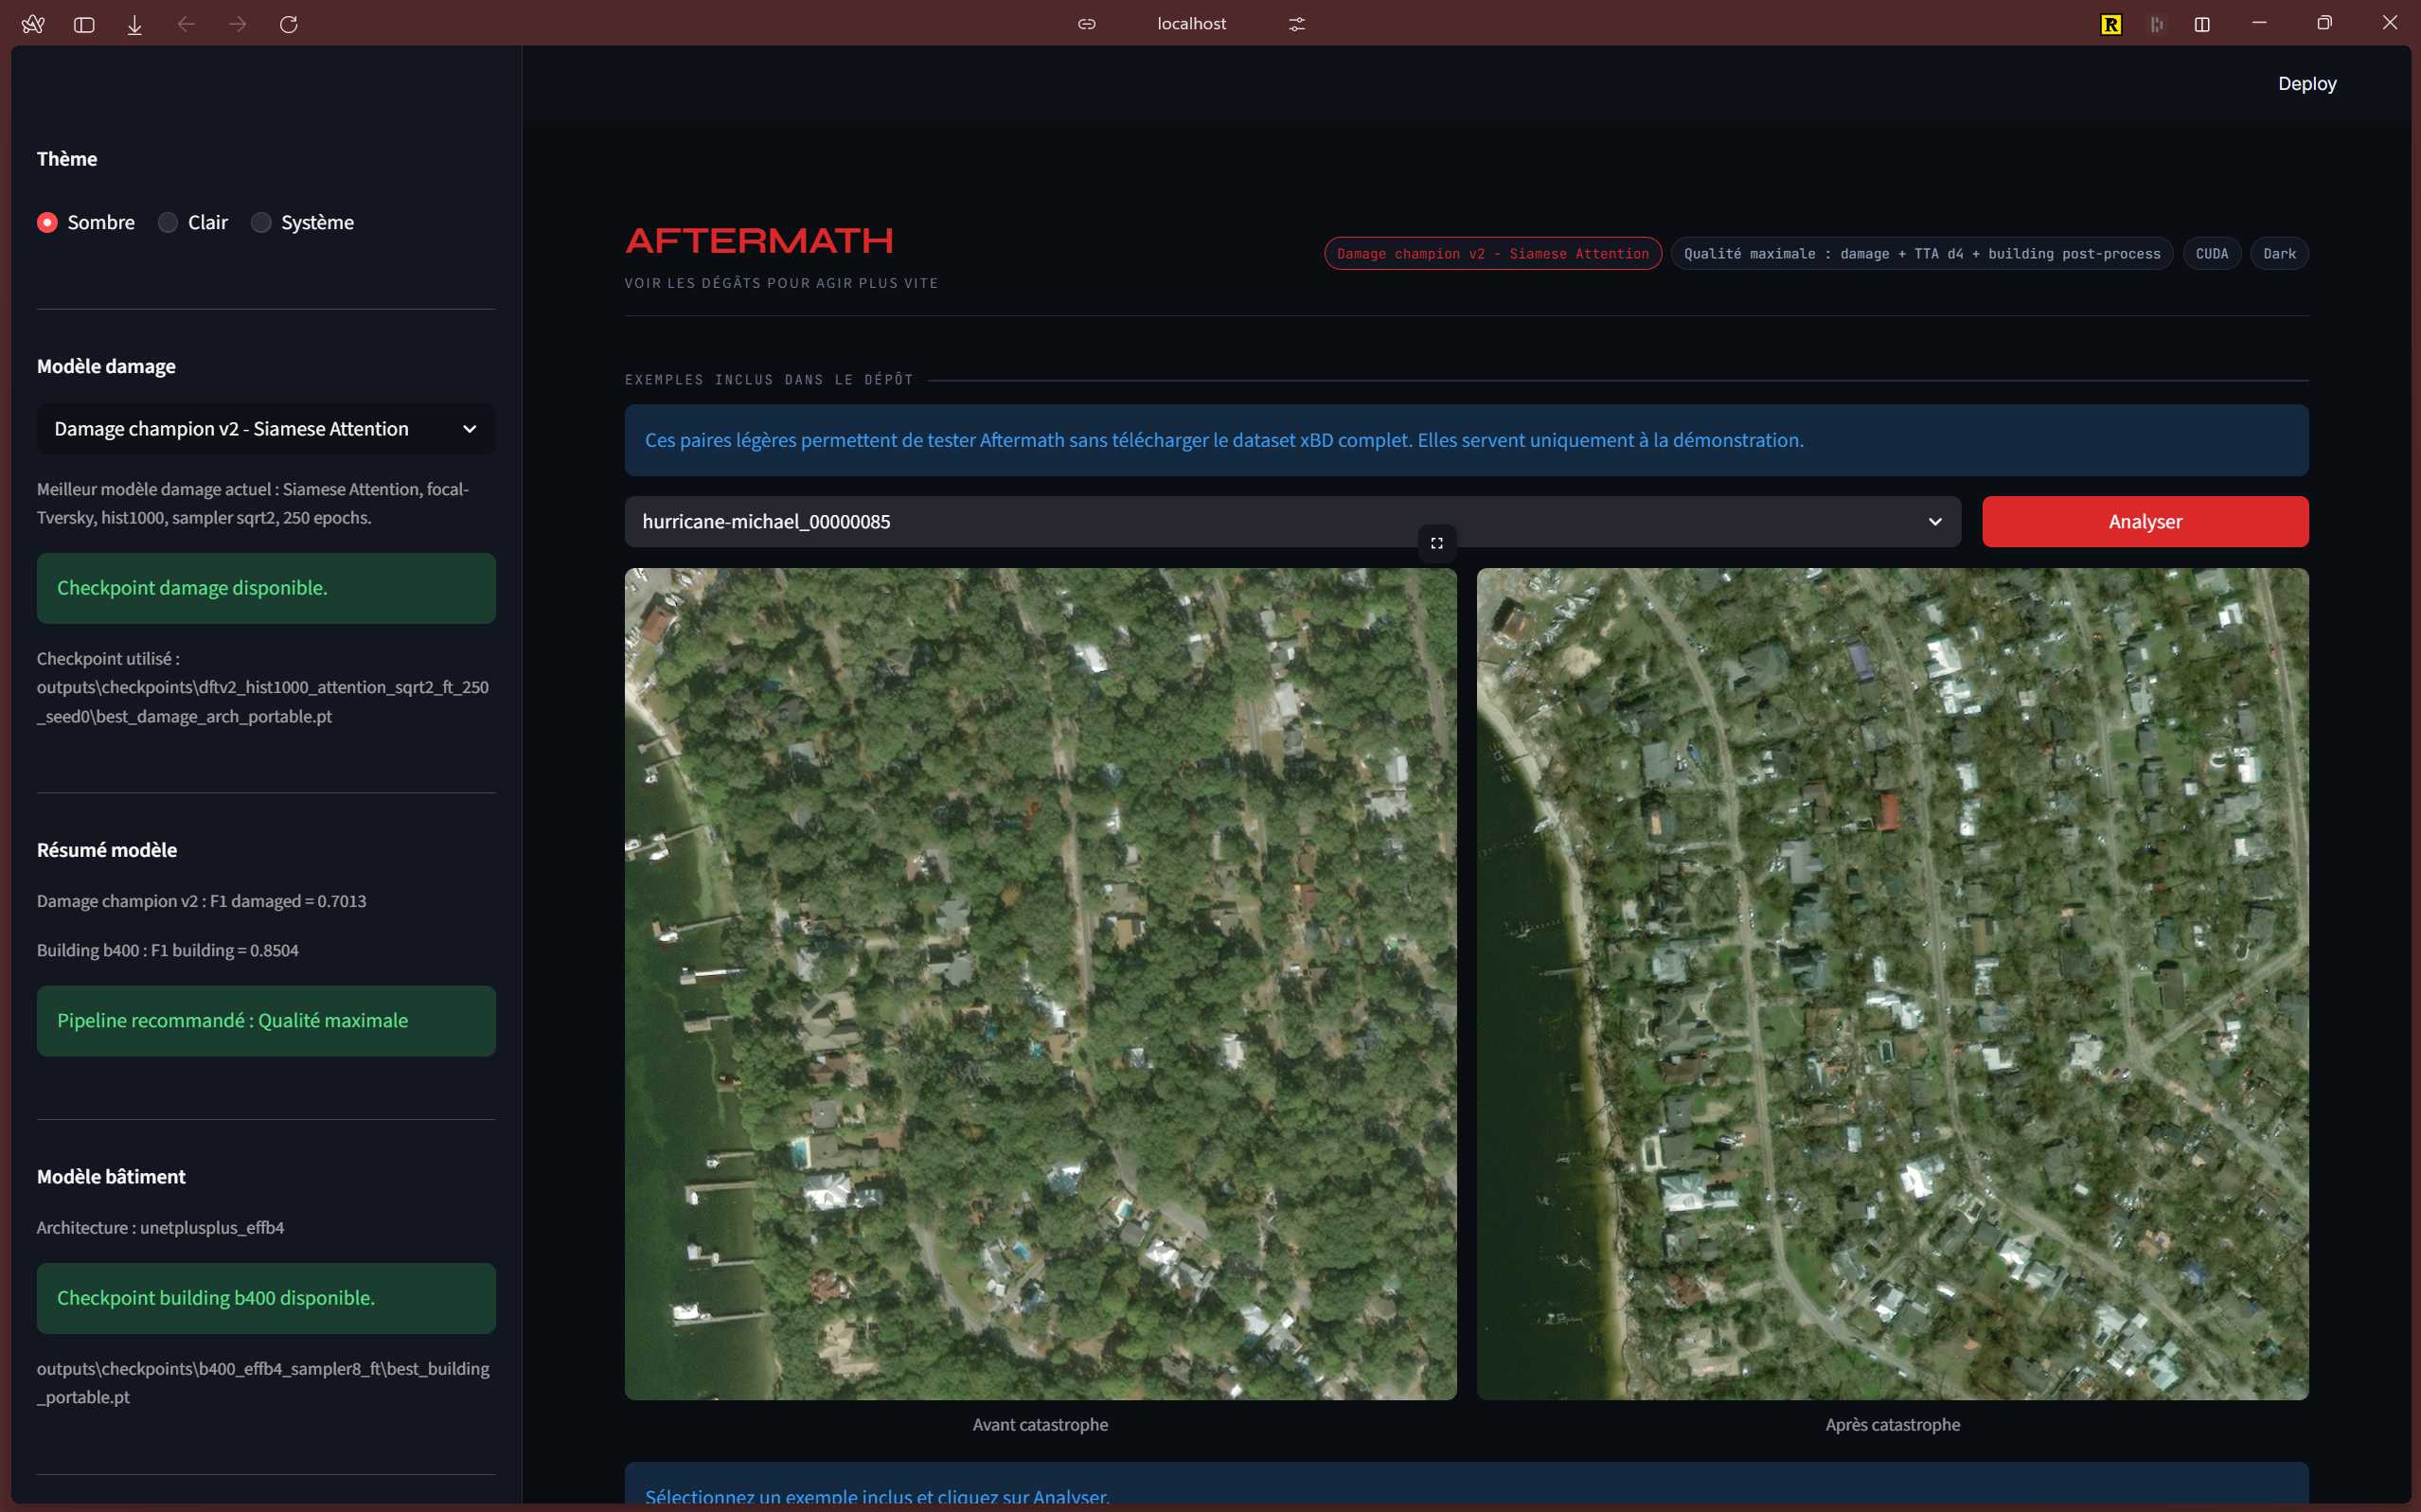
\includegraphics[width=0.92\textwidth]{docs/final_delivery/report_figures/app_interface_included_example.png}
    \caption{Interface principale de l'application Aftermath finale en mode \textbf{Exemples inclus}, avec l'exemple \texttt{hurricane-michael\_00000085} sélectionné.}
    \label{fig:interface_aftermath}
\end{figure}

\begin{figure}[H]
    \centering
    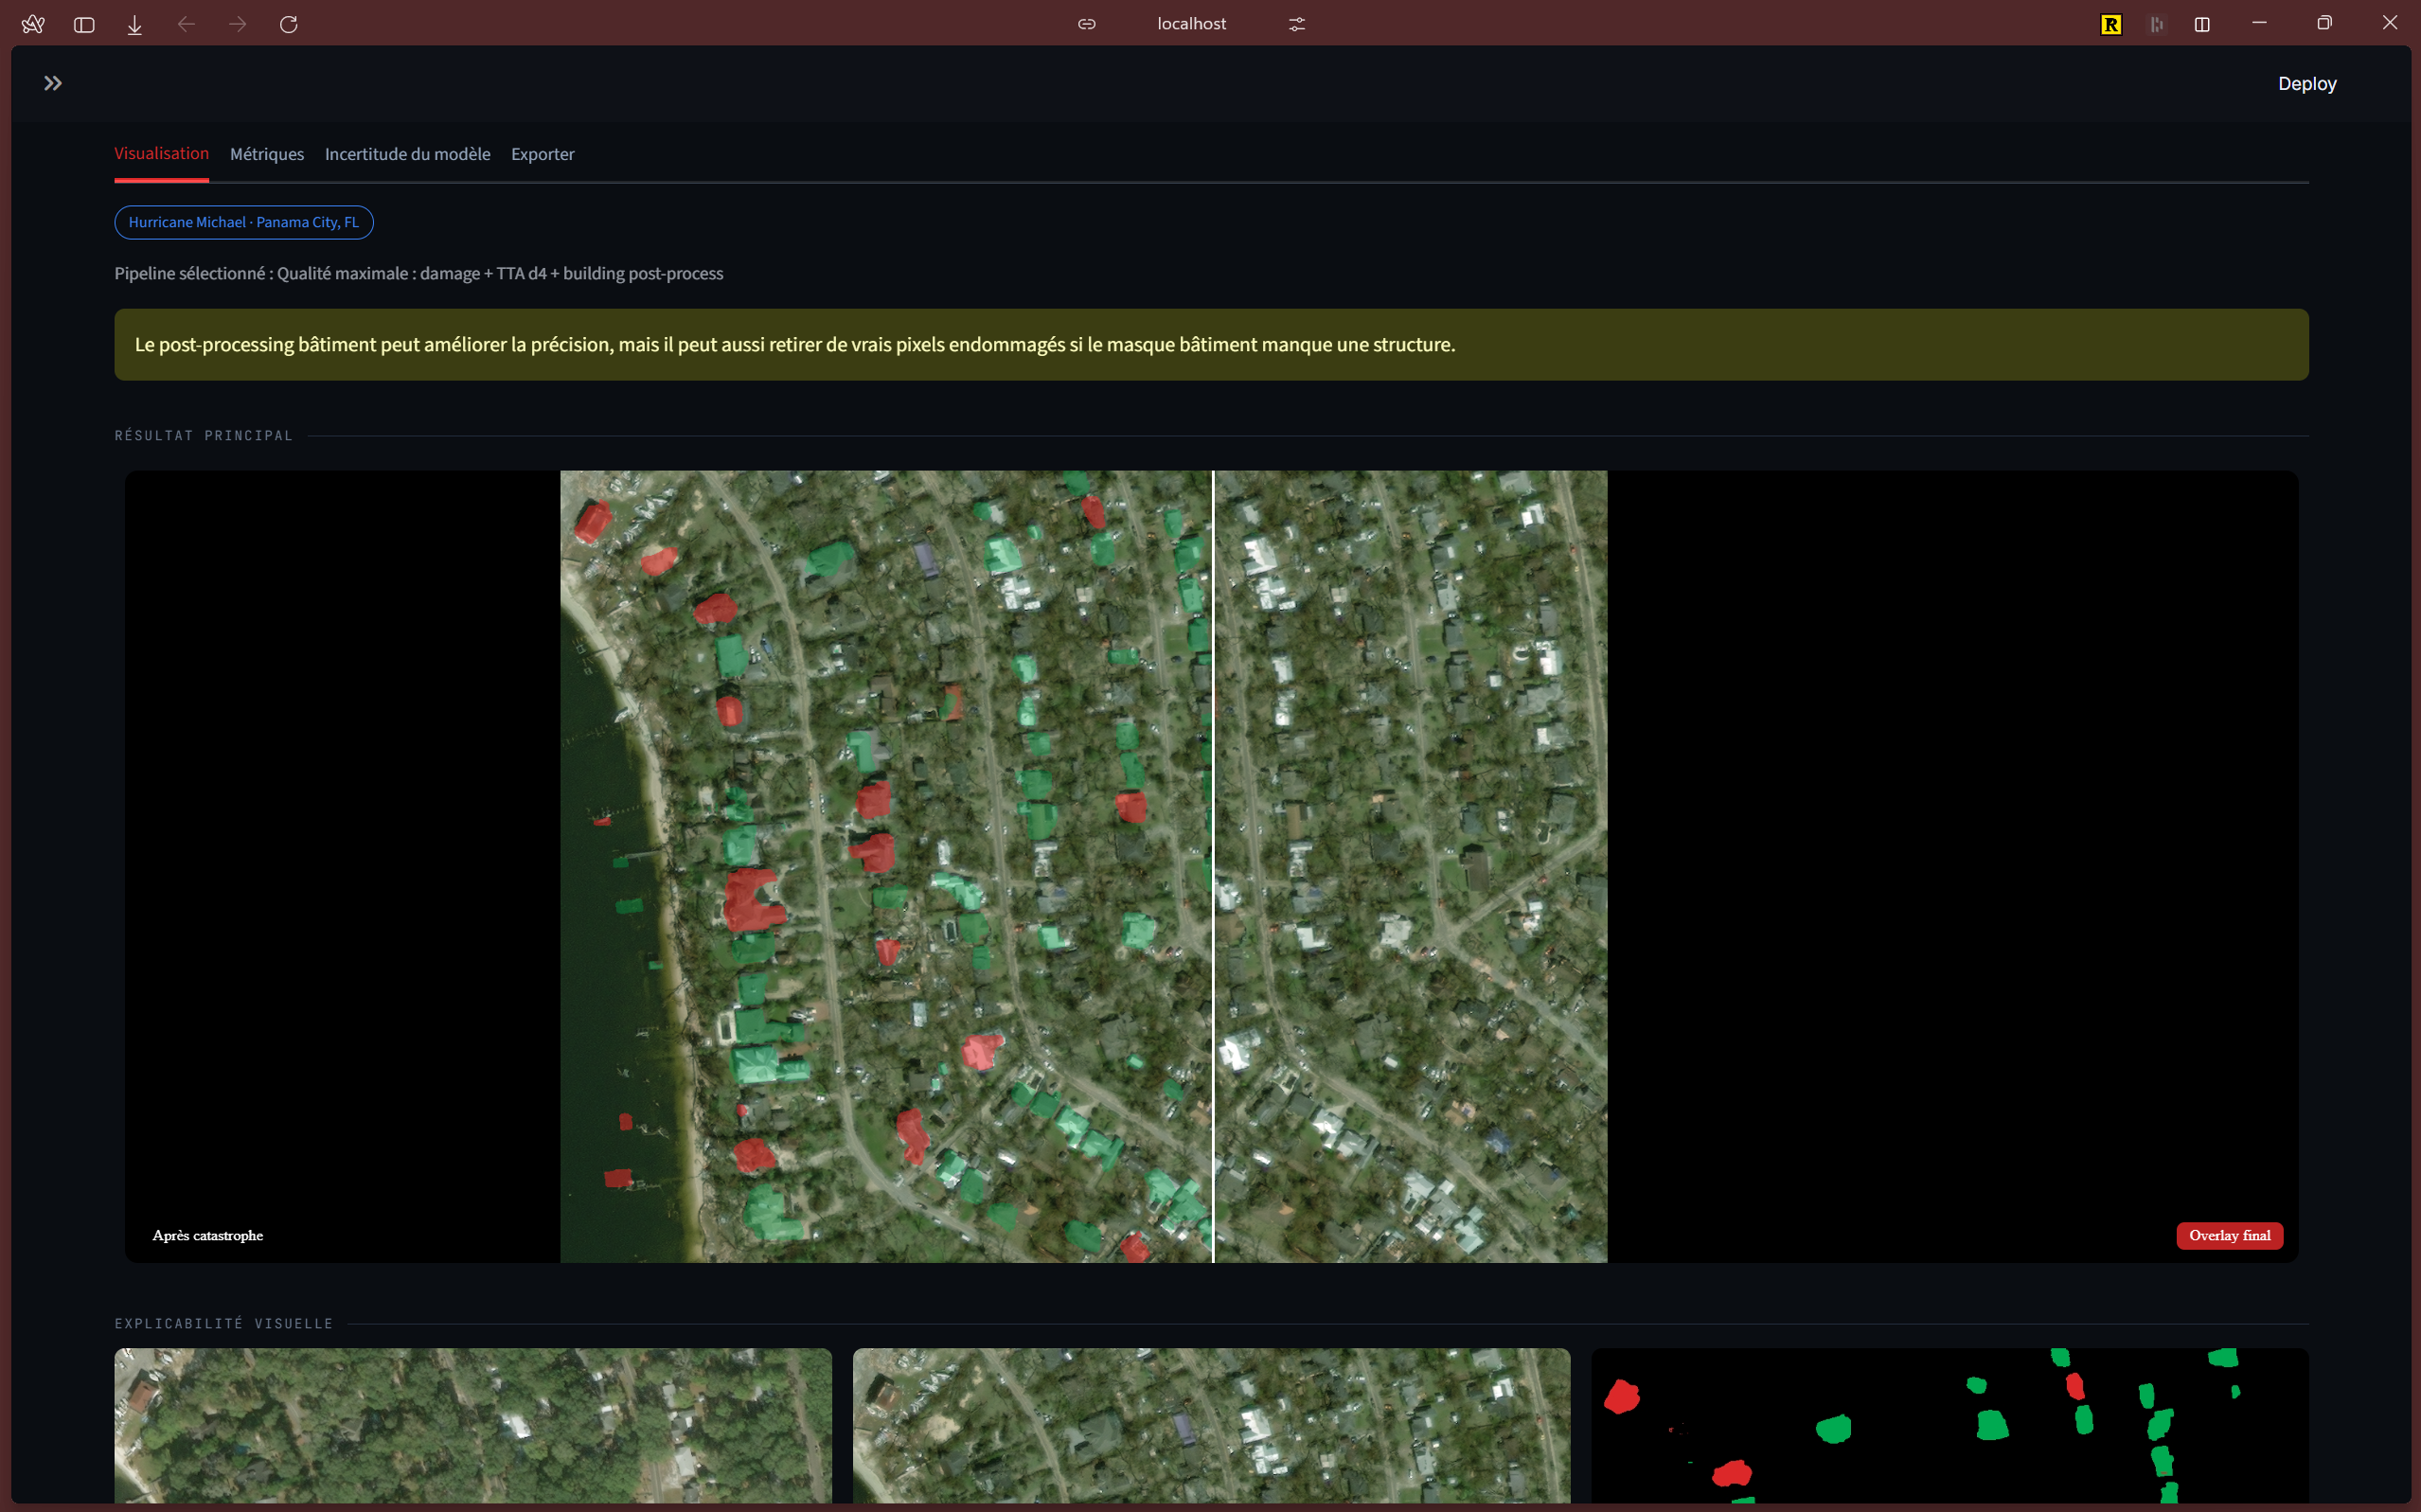
\includegraphics[width=0.92\textwidth]{docs/final_delivery/report_figures/app_visualisation_overlay.png}
    \caption{Onglet Visualisation de l'application finale : l'overlay final est affiché sur l'image post-catastrophe afin de rendre la prédiction directement interprétable.}
    \label{fig:app_visualisation_overlay}
\end{figure}

\begin{figure}[H]
    \centering
    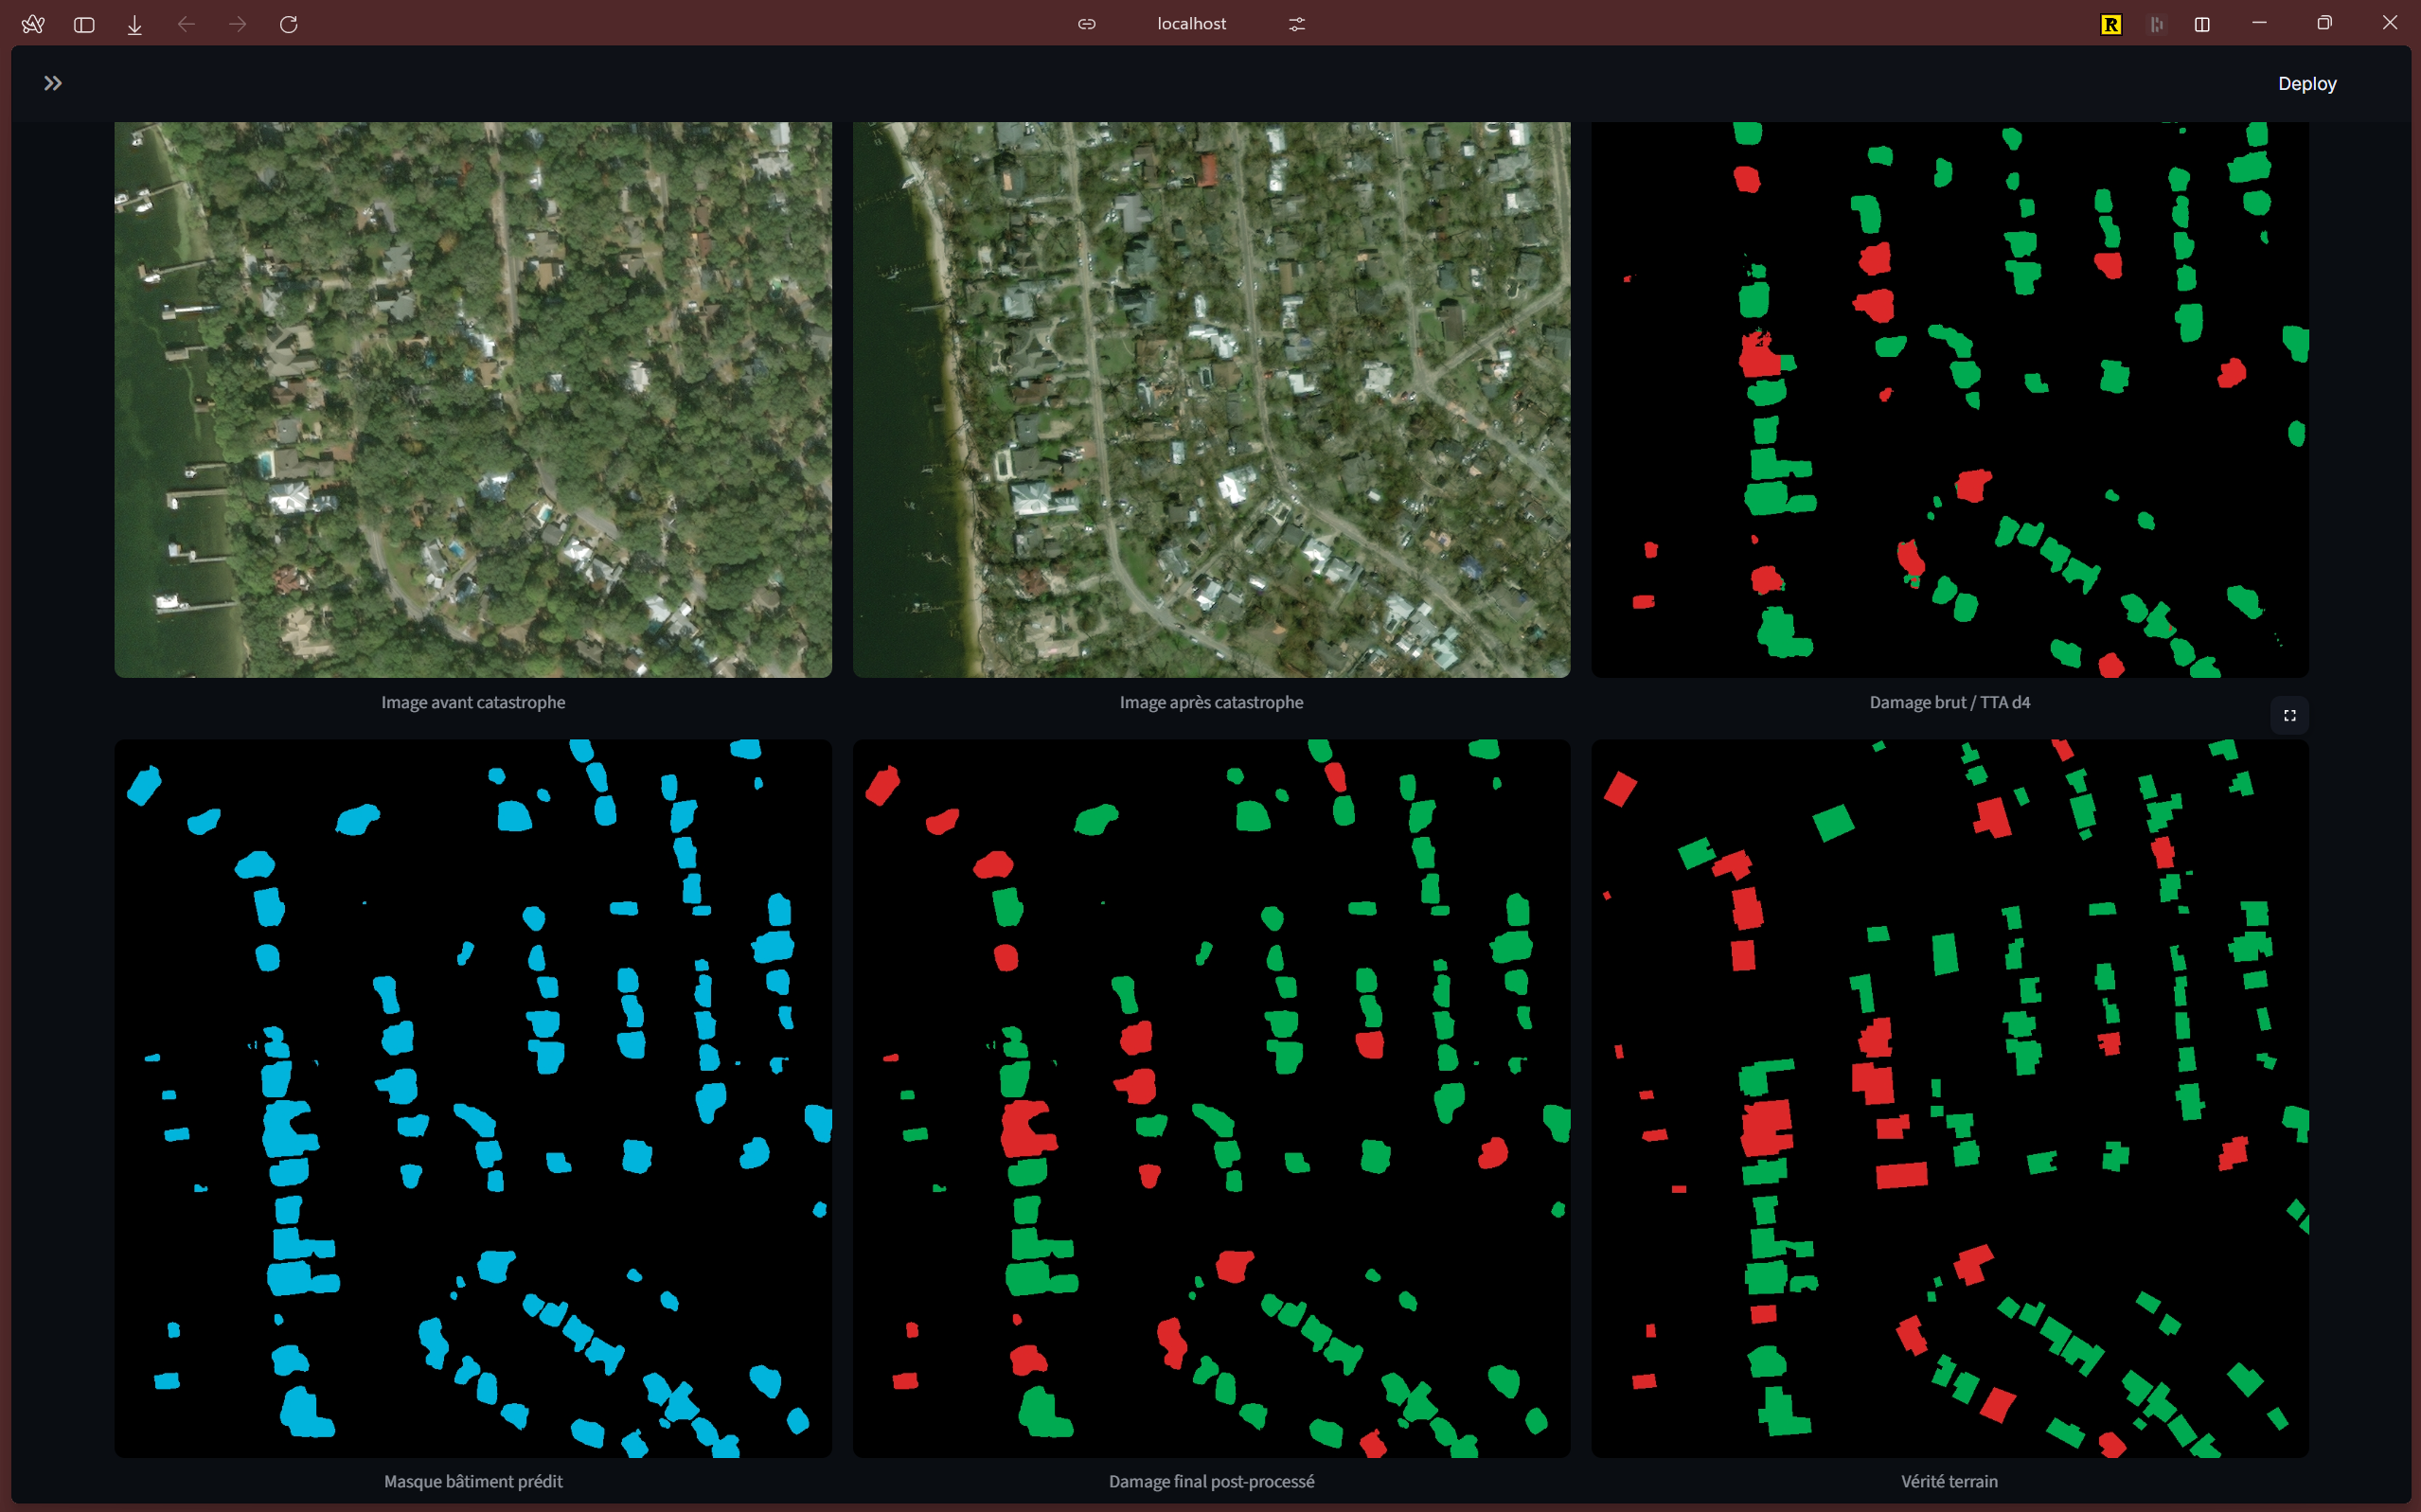
\includegraphics[width=0.92\textwidth]{docs/final_delivery/report_figures/app_intermediate_outputs.png}
    \caption{Sorties intermédiaires du pipeline : image avant, image après, damage brut, masque bâtiment, damage final post-traité et vérité terrain lorsque disponible.}
    \label{fig:app_intermediate_outputs}
\end{figure}

\section{Résultats}

\subsection{Métriques d'évaluation}

L'évaluation du modèle repose sur plusieurs métriques complémentaires. La \textit{Pixel Accuracy} mesure la proportion de pixels correctement prédits, mais elle doit être interprétée avec prudence dans notre cas, car la classe de fond est très majoritaire. Une forte précision globale peut donc masquer une mauvaise détection des bâtiments endommagés. Pour cette raison, les métriques principales du projet sont l'IoU et le F1-score sur la classe \textit{damaged}.

L'Intersection over Union (IoU) est plus informative pour la segmentation, car elle compare le recouvrement entre la prédiction et la vérité terrain :
\begin{equation}
    IoU = \frac{|Prediction \cap GroundTruth|}{|Prediction \cup GroundTruth|}
\end{equation}

La \textit{Mean IoU} correspond à la moyenne des IoU calculées sur les différentes classes. Le F1-score complète l'IoU en équilibrant précision et rappel. Dans un contexte de gestion de crise, ces deux dimensions sont importantes : un rappel élevé évite de manquer des bâtiments endommagés, tandis qu'une précision élevée évite de signaler trop de fausses zones critiques.

\begin{tcolorbox}[colback=blue!4,colframe=blue!50!black,title=Métriques locales dans l'application]
Les métriques affichées dans l'application pour un exemple donné sont locales à cette paire d'images ; les métriques globales du modèle sont présentées dans le tableau expérimental.
\end{tcolorbox}

\begin{figure}[H]
    \centering
    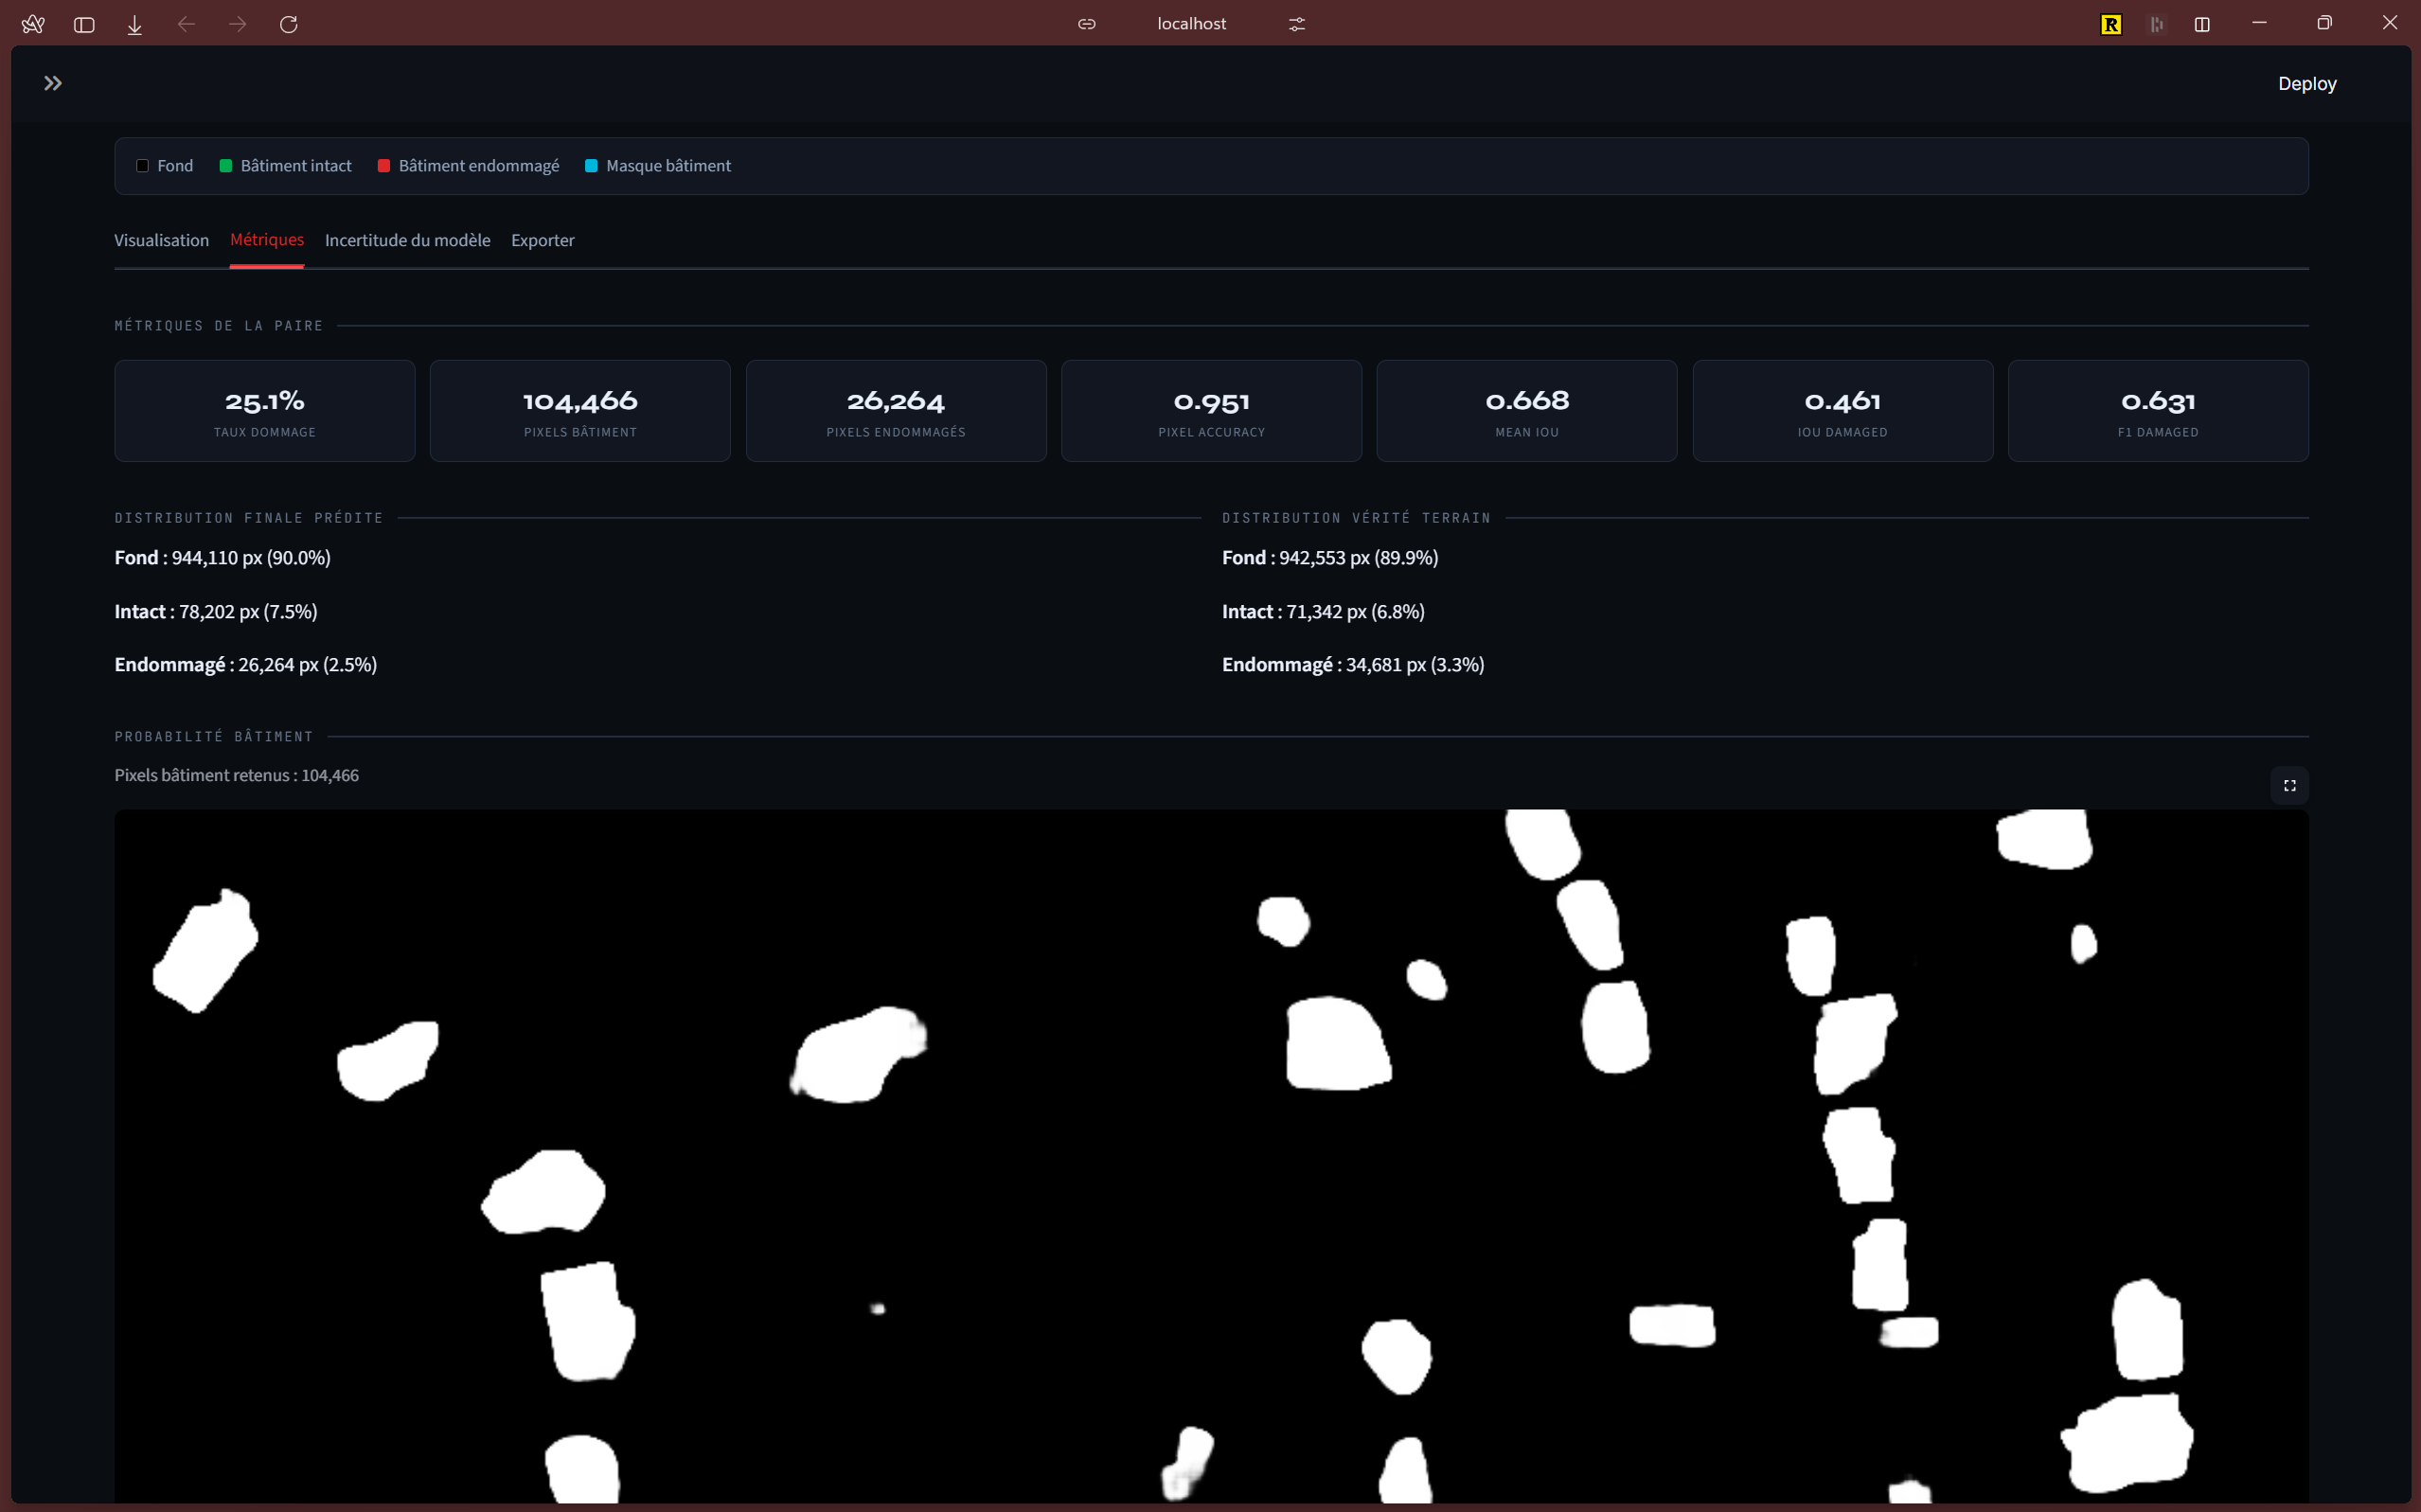
\includegraphics[width=0.9\textwidth]{docs/final_delivery/report_figures/app_metrics.png}
    \caption{Onglet Métriques de l'application finale. Ces scores servent à analyser une paire d'images lorsque la vérité terrain est disponible.}
    \label{fig:app_metrics}
\end{figure}

\subsection{Résultats expérimentaux}

Le tableau~\ref{tab:resultats_modeles} synthétise les principaux résultats damage retenus pour le rendu final. Les métriques sont calculées sur la formulation actuelle à trois classes : fond, bâtiment intact et bâtiment endommagé. Elles ne doivent donc pas être confondues avec le score officiel xView2 à cinq classes.

\begin{table}[H]
    \centering
    \begin{tabular}{|>{\raggedright\arraybackslash}m{5.2cm}|>{\centering\arraybackslash}m{2.1cm}|>{\centering\arraybackslash}m{2.1cm}|>{\centering\arraybackslash}m{2.1cm}|>{\raggedright\arraybackslash}m{3.5cm}|}
        \hline
        \textbf{Méthode} & \textbf{Mean IoU} & \textbf{IoU damaged} & \textbf{F1 damaged} & \textbf{Décision} \\
        \hline
        Baseline U-Net + TTA d4 & 0.6816 & 0.4612 & 0.6313 & Baseline forte; référence initiale stabilisée. \\ \hline
        Ancien champion Siamese Attention & 0.7073 & 0.5138 & 0.6788 & Première rupture nette par rapport au U-Net. \\ \hline
        \texttt{dftv2\_hist1000\_attention\_sqrt2\_ft\_250\_seed0} & 0.7283 & 0.5400 & 0.7013 & Champion intégré dans l'application finale. \\ \hline
        \texttt{dftv2\_hist1000\_attention\_sqrt4\_ft\_400\_seed0} & 0.7273 & 0.5406 & 0.7018 & Non retenu : gain marginal, modèle moins stabilisé côté intégration. \\ \hline
    \end{tabular}
    \caption{Comparaison finale des principaux modèles damage en formulation 3 classes.}
    \label{tab:resultats_modeles}
\end{table}

Le champion intégré dans l'application finale est donc le modèle \texttt{dftv2\_hist1000\_attention\_sqrt2\_ft\_250\_seed0}. Il repose sur une architecture \textbf{Siamese Attention}, une perte \textbf{focal-Tversky}, un split no-leak \textit{hist1000}, un sampler \textit{damage-sqrt} avec $\alpha=2$ et 250 époques d'entraînement. Le dernier run disponible, entraîné 400 époques avec $\alpha=4$, obtient un F1 damaged très légèrement supérieur (0.7018 contre 0.7013), mais le gain est trop faible pour justifier un changement tardif du prototype. Nous avons donc conservé le checkpoint déjà stabilisé, portable, versionné et testé dans l'application.

\subsection{Segmentation bâtiment}

Le modèle bâtiment est évalué séparément, car sa tâche est binaire : fond contre bâtiment. Son rôle dans le prototype est de contraindre le post-traitement damage aux zones bâties et de réduire les erreurs incohérentes hors bâtiment. Le meilleur modèle retenu est \texttt{b400\_effb4\_sampler8\_ft}, basé sur \textbf{U-Net++ EfficientNet-B4}, entraîné avec focal-Tversky et un sampler orienté bâtiment.

\begin{table}[H]
    \centering
    \begin{tabular}{|>{\raggedright\arraybackslash}m{5.5cm}|>{\centering\arraybackslash}m{3cm}|>{\centering\arraybackslash}m{3cm}|>{\raggedright\arraybackslash}m{3.2cm}|}
        \hline
        \textbf{Modèle bâtiment} & \textbf{IoU building} & \textbf{F1 building} & \textbf{Usage dans le prototype} \\
        \hline
        \texttt{b400\_effb4\_sampler8\_ft} & 0.7398 & 0.8504 & Masque bâtiment pour le post-traitement par composantes. \\ \hline
    \end{tabular}
    \caption{Résultat final du modèle de segmentation bâtiment intégré dans Aftermath.}
    \label{tab:resultats_building}
\end{table}

L'intérêt du modèle bâtiment est double. D'une part, il permet d'afficher explicitement où l'IA estime que les bâtiments se trouvent. D'autre part, il sert de garde-fou spatial pour la carte damage : une prédiction de dommage en pleine zone non bâtie est moins pertinente qu'une prédiction située sur une composante bâtiment.

\begin{figure}[H]
    \centering

    \begin{subfigure}[b]{0.32\textwidth}
        \centering
        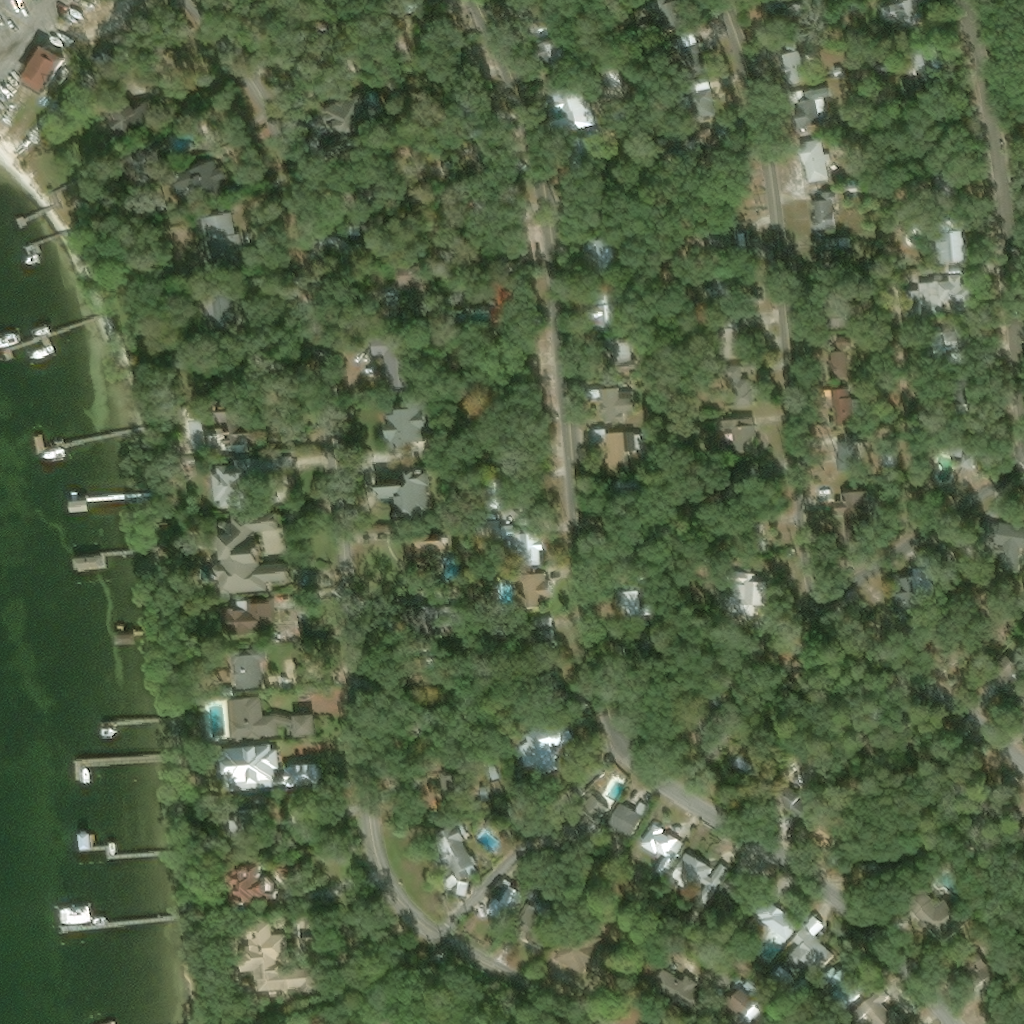
\includegraphics[width=\textwidth]{sample_data/demo_pairs/hurricane-michael_00000085/pre.png}
        \caption{Avant catastrophe}
    \end{subfigure}
    \hfill
    \begin{subfigure}[b]{0.32\textwidth}
        \centering
        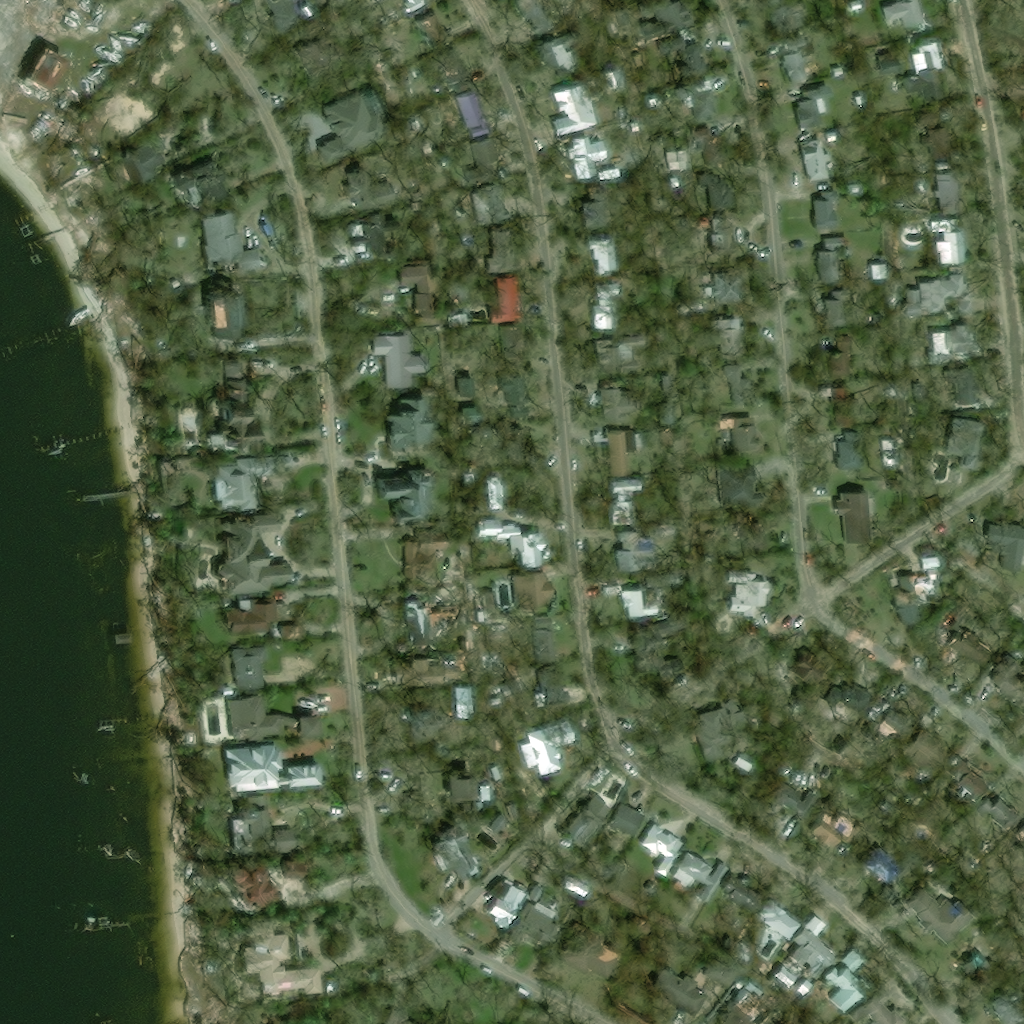
\includegraphics[width=\textwidth]{sample_data/demo_pairs/hurricane-michael_00000085/post.png}
        \caption{Après catastrophe}
    \end{subfigure}
    \hfill
    \begin{subfigure}[b]{0.32\textwidth}
        \centering
        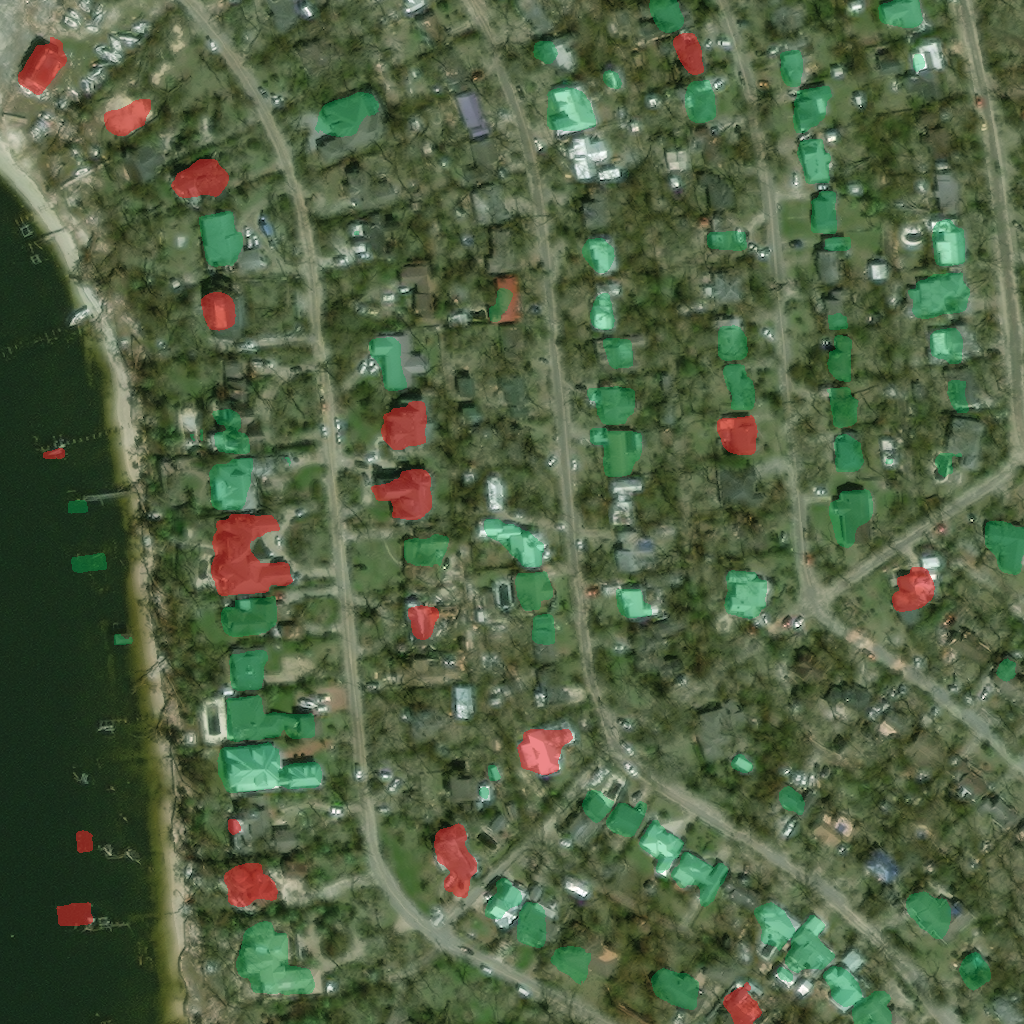
\includegraphics[width=\textwidth]{docs/final_delivery/report_figures/overlay_hurricane_michael_00000085.png}
        \caption{Overlay final}
    \end{subfigure}

    \caption{Exemple de prédiction générée par Aftermath sur la paire embarquée \texttt{hurricane-michael\_00000085}.}
    \label{fig:exemple_prediction}
\end{figure}

\subsection{Analyse}

Les résultats montrent une progression nette entre la baseline U-Net et le modèle final. Le F1 damaged passe de 0.6313 à 0.7013, tandis que l'IoU damaged progresse de 0.4612 à 0.5400. Cette amélioration est importante, car la classe \textit{damaged} est la plus rare et la plus difficile : elle combine localisation bâtiment, comparaison temporelle avant/après et classification visuelle du niveau de dommage.

L'analyse qualitative reste néanmoins indispensable. Certaines erreurs proviennent d'un décalage entre l'image pré-catastrophe et l'image post-catastrophe, d'ombres, de textures de toiture ambiguës ou de bâtiments partiellement masqués. D'autres erreurs concernent les contours : une prédiction peut être visuellement utile mais perdre des points d'IoU si le masque est légèrement décalé par rapport à la vérité terrain. Enfin, le post-traitement par bâtiment peut supprimer des faux positifs hors bâtiment, mais il peut aussi supprimer de vrais dommages si le masque bâtiment manque une structure. C'est pour cela que l'application affiche à la fois le damage brut, le masque bâtiment et le damage final post-traité.

Le prototype doit donc être compris comme un outil d'aide à la décision. Il accélère une première lecture de la zone et met en évidence des hypothèses de dégâts, mais il ne remplace pas l'analyse d'un expert SIG, d'un analyste humanitaire ou d'une cellule de crise.

\section{Parcours utilisateur}

Pour comprendre l'utilisation de notre plateforme Aftermath au quotidien, nous pouvons suivre le parcours type d'un analyste en gestion de crise lors d'une alerte.

Dès l'ouverture de l'application, l'opérateur fait face à une interface divisée en deux zones : un menu de configuration à gauche et un espace de visualisation au centre. L'utilisateur commence par choisir la source des données. Pour une démonstration rapide, il sélectionne une paire embarquée dans \texttt{sample\_data/demo\_pairs/}. Pour un test libre, il glisse-dépose directement ses propres fichiers d'images satellites avant et après l'événement. Si le dataset xBD complet est installé localement, il peut aussi parcourir les exemples du split de test ou de validation.

Une fois les images chargées, l'opérateur choisit le pipeline d'inférence. Pour la démonstration finale, le mode recommandé est le mode qualité maximale : modèle damage Siamese Attention, TTA d4, segmentation bâtiment U-Net++ EfficientNet-B4 et post-traitement \textit{component majority}. L'application indique aussi si les checkpoints portables nécessaires sont bien disponibles.

Un clic sur le bouton de lancement démarre l'analyse. Quelques secondes plus tard, l'espace central se met à jour. L'opérateur visualise l'overlay final sur l'image post-catastrophe, puis peut inspecter les sorties intermédiaires : image avant, image après, damage brut, masque bâtiment, damage final post-traité et vérité terrain lorsqu'elle existe. En cas de doute sur un secteur, l'utilisateur bascule sur l'onglet d'incertitude pour voir les zones où le modèle hésite le plus. Le parcours se termine par l'analyse des statistiques globales et le téléchargement d'exports PNG/JSON.

\section{Livrable final et reproductibilité}

Le rendu final est organisé comme un dépôt GitHub clé en main. Il contient le code source, l'application Streamlit finale, les deux checkpoints portables nécessaires au prototype, quelques exemples embarqués et une documentation technique d'installation. Le dataset xBD complet n'est pas inclus, car il est volumineux; il reste optionnel pour reproduire l'ensemble des évaluations.

Les fichiers essentiels du prototype sont :
\begin{itemize}
    \item \texttt{app/streamlit\_app.py} : application finale;
    \item \texttt{sample\_data/demo\_pairs/} : exemples pré/post-catastrophe utilisables sans dataset complet;
    \item \texttt{outputs/checkpoints/dftv2\_hist1000\_attention\_sqrt2\_ft\_250\_seed0/best\_damage\_arch\_portable.pt} : checkpoint damage intégré;
    \item \texttt{outputs/checkpoints/b400\_effb4\_sampler8\_ft/best\_building\_portable.pt} : checkpoint building intégré.
\end{itemize}

La commande principale de lancement est :
\begin{lstlisting}
python -m streamlit run app/streamlit_app.py
\end{lstlisting}

Cette organisation permet à un évaluateur de tester la solution sans relancer d'entraînement et sans télécharger l'intégralité des sorties expérimentales.

\section{Limites du projet}

Malgré l'intérêt de notre solution, deux principales limites techniques et opérationnelles doivent être soulignées.

La première concerne le traitement d'images réelles en dehors du dataset d'entraînement. Notre modèle a été entraîné sur des images xBD standardisées, recadrées et nettoyées. Dans la réalité, les images satellites brutes récupérées en urgence peuvent présenter des angles de prise de vue différents, des résolutions variées ou des conditions météorologiques défavorables comme des nuages ou des ombres portées importantes. Bien que la data augmentation permette d'intégrer une certaine variabilité lors de l'entraînement, ces différences visuelles peuvent encore perturber l'IA et générer de fausses détections.

La seconde limite réside dans le fait que notre modèle actuel fonctionne sur une simplification à trois classes : fond, bâtiments intacts et bâtiments endommagés. Cette approche élimine les nuances de l'échelle internationale xBD qui sépare les dégâts mineurs des dégâts majeurs et des bâtiments détruits \cite{xbd}. Sur le terrain, un bâtiment avec un toit légèrement abîmé et un édifice totalement effondré demandent des interventions différentes, ce que notre modèle ne peut pas encore distinguer précisément.

Une troisième limite concerne l'intégration géographique. Le prototype final exporte des images PNG et un fichier JSON descriptif, mais il ne produit pas encore de GeoJSON, GeoTIFF, Shapefile, projet QGIS/ArcGIS, API publique ou géoréférencement opérationnel. Ces fonctions seraient nécessaires pour une utilisation terrain complète dans une chaîne SIG professionnelle.

\section{Perspectives}

Les perspectives de développement pour ce projet se concentrent sur deux axes : l'amélioration algorithmique et l'intégration cartographique professionnelle.

Sur le plan de l'IA, la suite logique consiste à réintégrer l'échelle complète à cinq classes du dataset xBD. Séparer les sinistres mineurs, majeurs et totaux permettra d'affiner la détection, offrant ainsi des cartes plus précises pour l'évaluation des coûts de reconstruction et le tri des priorités de secours. Des travaux plus récents sur l'évaluation des dégâts multi-catastrophes montrent d'ailleurs que la segmentation et la classification des dommages restent des tâches actives en recherche appliquée \cite{deepdamagenet}.

Sur le plan opérationnel, la perspective principale est l'intégration aux Systèmes d'Information Géographique (SIG). Les exports actuels PNG/JSON sont suffisants pour une démonstration visuelle et pour conserver les statistiques d'une inférence, mais ils ne constituent pas encore des exports SIG complets. Une évolution future consisterait à produire des fichiers GeoJSON, \textit{Shapefile} (.shp) ou \textit{GeoTIFF} géoréférencés. Le format GeoTIFF permet notamment d'intégrer des informations de géoréférencement directement dans un fichier TIFF, ce qui le rend adapté aux échanges d'images géospatiales \cite{geotiff}. Un cartographe pourrait alors ouvrir les prédictions de l'IA dans des logiciels comme QGIS ou ArcGIS, les superposer aux réseaux routiers existants et extraire les coordonnées nécessaires aux équipes terrain \cite{qgis}.

\section{Conclusion}

En conclusion, ce projet a permis de concevoir une chaîne complète d'évaluation automatisée des dommages après une catastrophe naturelle. À partir du dataset xBD, nous avons mis en place un pipeline de traitement reliant la préparation des données, l'entraînement de modèles de segmentation, le post-traitement des prédictions et la visualisation dans une interface utilisateur.

Le développement de la plateforme Aftermath concrétise ces efforts techniques à travers un outil visuel, accessible et rapide, capable de traduire des images satellites complexes en cartes de crise exploitables. L'approche retenue repose sur des méthodes reconnues en segmentation, notamment U-Net, U-Net++, les architectures siamoises et les fonctions de perte adaptées aux données déséquilibrées \cite{unet,unetplusplus,siamunet_attn,dice_loss,tversky_loss}.

Bien qu'il reste des étapes à franchir pour l'intégration SIG, le géoréférencement opérationnel et l'affinage de la classification des dégâts, ce prototype démontre le potentiel de l'apprentissage profond pour épauler les organisations humanitaires et optimiser la prise de décision en situation d'urgence.

\newpage

\begin{thebibliography}{15}

\bibitem{xbd}
R. Gupta, R. Hosfelt, S. Sajeev, N. Patel, B. Goodman, J. Doshi, E. Heim, H. Choset et M. Gaston,
\textit{xBD: A Dataset for Assessing Building Damage from Satellite Imagery},
arXiv:1911.09296, 2019.

\bibitem{xview2_multitemporal}
E. Weber et H. Kané,
\textit{Building Disaster Damage Assessment in Satellite Imagery with Multi-Temporal Fusion},
arXiv:2004.05525, 2020.

\bibitem{siamunet_attn}
H. Hao, S. Baireddy, E. R. Bartusiak, L. Konz, K. LaTourette, M. Gribbons, M. Chan, M. L. Comer et E. J. Delp,
\textit{An Attention-Based System for Damage Assessment Using Satellite Imagery},
arXiv:2004.06643, 2020.

\bibitem{unet}
O. Ronneberger, P. Fischer et T. Brox,
\textit{U-Net: Convolutional Networks for Biomedical Image Segmentation},
arXiv:1505.04597, 2015.

\bibitem{unetplusplus}
Z. Zhou, M. M. R. Siddiquee, N. Tajbakhsh et J. Liang,
\textit{UNet++: A Nested U-Net Architecture for Medical Image Segmentation},
arXiv:1807.10165, 2018.

\bibitem{dice_loss}
F. Milletari, N. Navab et S.-A. Ahmadi,
\textit{V-Net: Fully Convolutional Neural Networks for Volumetric Medical Image Segmentation},
arXiv:1606.04797, 2016.

\bibitem{tversky_loss}
S. S. M. Salehi, D. Erdogmus et A. Gholipour,
\textit{Tversky Loss Function for Image Segmentation Using 3D Fully Convolutional Deep Networks},
arXiv:1706.05721, 2017.

\bibitem{focal_tversky}
N. Abraham et N. M. Khan,
\textit{A Novel Focal Tversky Loss Function with Improved Attention U-Net for Lesion Segmentation},
arXiv:1810.07842, 2018.

\bibitem{pytorch}
A. Paszke et al.,
\textit{PyTorch: An Imperative Style, High-Performance Deep Learning Library},
arXiv:1912.01703, 2019.

\bibitem{streamlit}
Streamlit,
\textit{Streamlit Documentation},
Snowflake Inc., documentation officielle consultée en juin 2026.

\bibitem{slurm}
SchedMD,
\textit{Slurm Workload Manager Documentation},
documentation officielle consultée en juin 2026.

\bibitem{qgis}
QGIS Project,
\textit{QGIS User Guide},
documentation officielle consultée en juin 2026.

\bibitem{geotiff}
Open Geospatial Consortium,
\textit{OGC GeoTIFF Standard},
version 1.1, OGC Document No. 19-008r4, 2019.

\bibitem{deepdamagenet}
I. Alisjahbana, J. Li, B. Strong et Y. Zhang,
\textit{DeepDamageNet: A Two-Step Deep-Learning Model for Multi-Disaster Building Damage Segmentation and Classification Using Satellite Imagery},
arXiv:2405.04800, 2024.

\end{thebibliography}

\end{document}
